% ==========================================
% BAB V IMPLEMENTASI
% ==========================================
\cleardoublepage
\chapter{IMPLEMENTASI SISTEM \textit{BUSINESS INTELLIGENCE CHATBOT}}
\label{chap:implementasi}

Bab ini menyajikan implementasi sistem \textit{Business Intelligence} berbasis \textit{rule-based chatbot} yang telah dirancang pada bab sebelumnya. Pembahasan mencakup arsitektur sistem yang diimplementasikan, implementasi setiap komponen utama, serta integrasi antar-komponen menjadi satu kesatuan sistem yang fungsional.

\section{Arsitektur Sistem Terimplementasi}
\label{sec:arsitektur-terimplementasi}

Sistem BrightAI diimplementasikan dengan arsitektur tiga lapis (\textit{three-tier architecture}) yang memisahkan tanggung jawab setiap komponen secara jelas. Ketiga lapis tersebut adalah sebagai berikut.

\begin{enumerate}
    \item \textbf{\textit{Frontend} (React.js)}: Antarmuka pengguna berbasis web yang menyediakan fitur percakapan \textit{chatbot}, panel peramalan, dan manajemen profil pengguna. \textit{Frontend} berjalan pada porta 3000 dan berkomunikasi dengan \textit{backend} melalui \textit{RESTful API}.
    \item \textbf{\textit{Backend} (Node.js/Express)}: Peladen utama yang menangani autentikasi, manajemen sesi, eksekusi mesin aturan (\textit{rule engine}), klasifikasi maksud (\textit{intent classification}), pembangkitan bahasa alami (NLG), serta komunikasi dengan basis data Oracle. \textit{Backend} berjalan pada porta 3001.
    \item \textbf{Layanan \textit{Machine Learning} (FastAPI/PyTorch)}: Layanan terpisah yang menangani pelatihan dan inferensi model peramalan deret waktu berbasis GRU dan LSTM. Layanan ini berjalan pada porta 8000 dan diakses oleh \textit{backend} melalui permintaan HTTP internal.
\end{enumerate}

Ketiga lapis terhubung ke Oracle Database yang berfungsi ganda melalui dua skema terpisah: (1) skema \texttt{DWH\_MOIS} sebagai \textit{Enterprise Data Warehouse} (DWH)\label{abbr:DWH} yang menyimpan lima tabel domain analitik dengan prefiks \texttt{BRIGHTAI\_} (\texttt{BRIGHTAI\_SALES}, \texttt{BRIGHTAI\_REVENUE}, \texttt{BRIGHTAI\_TARGET}, \texttt{BRIGHTAI\_DAPROS}, \texttt{BRIGHTAI\_CT0\_NAL}); dan (2) skema \texttt{USR\_RPT} yang menyimpan data operasional sistem, meliputi tabel pengguna (\texttt{BRIGHTAI\_USER}), riwayat percakapan (\texttt{BRIGHTAI\_CHAT}), dan sesi (\texttt{BRIGHTAI\_SESSION}).

\section{Implementasi \textit{Backend} (Node.js/Express)}
\label{sec:impl-backend}

\textit{Backend} sistem diimplementasikan menggunakan Node.js dengan \textit{framework} Express.js sebagai fondasi \textit{RESTful API}. Berkas utama \texttt{server.js} menginisialisasi aplikasi Express, mengonfigurasi \textit{middleware}, mendaftarkan rute API, serta mengelola siklus hidup koneksi basis data.

\subsection{Struktur Proyek \textit{Backend}}

Proyek \textit{backend} diorganisasi menggunakan pola arsitektur MVC (\textit{Model-View-Controller}) yang dimodifikasi menjadi struktur berlapis. Tabel~\ref{tab:struktur-backend} menyajikan struktur direktori utama.

\begin{longtable}{|p{4.5cm}|p{8.5cm}|}
\caption{Struktur Direktori Proyek \textit{Backend}} \label{tab:struktur-backend} \\
\hline
\textbf{Direktori/Berkas} & \textbf{Fungsi} \\
\hline
\endfirsthead
\hline
\textbf{Direktori/Berkas} & \textbf{Fungsi} \\
\hline
\endhead
\hline
\endfoot
\texttt{server.js} & Titik masuk utama aplikasi: inisialisasi Express, \textit{middleware}, rute, dan koneksi basis data \\
\hline
\texttt{config/database.js} & Konfigurasi koneksi Oracle Database, \textit{connection pooling}, dan eksekutor kueri \\
\hline
\texttt{src/controllers/} & Penangan permintaan (\textit{request handler}): \texttt{authController.js} dan \texttt{chatController.js} \\
\hline
\texttt{src/models/} & Model data untuk pengguna, riwayat percakapan, dan sesi \\
\hline
\texttt{src/routes/} & Definisi rute API: autentikasi, \textit{chat}, sesi, dan peramalan \\
\hline
\texttt{src/rules/engine/} & Mesin aturan, klasifikasi maksud, pemroses kueri, dan pembangkit bahasa alami \\
\hline
\texttt{src/rules/databases/} & Definisi aturan per domain basis data \\
\hline
\texttt{src/rules/config/} & Registri aturan dan konfigurasi pemetaan tabel \\
\hline
\texttt{src/middleware/} & \textit{Middleware} autentikasi JWT dan penanganan kesalahan \\
\hline
\texttt{src/utils/} & Utilitas: \textit{logger}, \textit{cache}, dan fungsi pembantu \\
\hline
\end{longtable}


\subsection{Konfigurasi \textit{Middleware} Keamanan}

Sistem mengimplementasikan beberapa lapisan \textit{middleware} keamanan pada Express.js untuk melindungi API dari ancaman umum. Konfigurasi \textit{middleware} yang diterapkan mencakup:

\begin{enumerate}
    \item \textbf{Helmet}: Mengatur tajuk HTTP keamanan (\textit{security headers}) untuk mencegah serangan seperti \textit{Cross-Site Scripting} (XSS) dan \textit{clickjacking}.
    \item \textbf{CORS\label{abbr:CORS} (\textit{Cross-Origin Resource Sharing})}: Mengizinkan permintaan lintas-asal dari \textit{frontend} yang berjalan pada domain berbeda.
    \item \textbf{\textit{Rate Limiter}}: Membatasi jumlah permintaan per alamat IP menjadi maksimal 100 permintaan per 15 menit untuk mencegah serangan \textit{brute force} dan \textit{Denial of Service} (DoS).
    \item \textbf{Pembatasan Ukuran \textit{Payload}}: Membatasi ukuran badan permintaan JSON menjadi maksimal 10 MB.
\end{enumerate}

\subsection{Koneksi Oracle Database}
\label{subsec:koneksi-oracle}

Koneksi ke Oracle Database dikelola melalui modul \texttt{config/database.js} menggunakan pustaka \texttt{node-oracledb}. Satu \textit{connection pool} melayani akses ke kedua skema: \texttt{DWH\_MOIS} untuk kueri analitik dan \texttt{USR\_RPT} untuk operasi autentikasi serta manajemen sesi. Konfigurasi \textit{pool} disajikan pada Tabel~\ref{tab:pool-config}.

\begin{table}[h]
\centering
\caption{Konfigurasi \textit{Connection Pool} Oracle Database}
\label{tab:pool-config}
\begin{tabular}{|p{4cm}|c|p{6cm}|}
\hline
\textbf{Parameter} & \textbf{Nilai} & \textbf{Keterangan} \\
\hline
\texttt{poolMin} & 2 & Jumlah koneksi minimum yang dipertahankan \\
\hline
\texttt{poolMax} & 10 & Jumlah koneksi maksimum yang diizinkan \\
\hline
\texttt{poolIncrement} & 1 & Penambahan koneksi per permintaan baru \\
\hline
\texttt{connectTimeout} & 10 detik & Batas waktu koneksi awal \\
\hline
\end{tabular}
\end{table}

Modul ini juga menyediakan fungsi \texttt{executeQuery} yang menangani eksekusi kueri SQL dengan format keluaran objek (\texttt{OUT\_FORMAT\_OBJECT}), penanganan tipe data CLOB secara otomatis, serta penutupan koneksi yang aman melalui blok \texttt{finally}. Setiap baris hasil kueri yang mengandung CLOB diproses secara asinkron menggunakan \textit{stream} untuk mencegah kebocoran memori.

\subsection{Rute API (\textit{API Routes})}

\textit{Backend} menyediakan empat kelompok rute API utama yang disajikan pada Tabel~\ref{tab:api-routes}.

\begin{longtable}{|p{1.5cm}|p{4cm}|p{7cm}|}
\caption{Rute API Sistem BrightAI} \label{tab:api-routes} \\
\hline
\textbf{Metode} & \textbf{\textit{Endpoint}} & \textbf{Fungsi} \\
\hline
\endfirsthead
\hline
\textbf{Metode} & \textbf{\textit{Endpoint}} & \textbf{Fungsi} \\
\hline
\endhead
\hline
\endfoot
POST & \texttt{/api/auth/register} & Registrasi pengguna baru \\
\hline
POST & \texttt{/api/auth/login} & Autentikasi dan penerbitan token JWT \\
\hline
GET & \texttt{/api/auth/profile} & Mengambil profil pengguna (memerlukan token) \\
\hline
PUT & \texttt{/api/auth/profile} & Memperbarui profil pengguna \\
\hline
PUT & \texttt{/api/auth/password} & Mengubah kata sandi \\
\hline
POST & \texttt{/api/chat/message} & Mengirim pesan ke \textit{chatbot} dan menerima respons \\
\hline
GET & \texttt{/api/chat/history} & Mengambil riwayat percakapan pengguna \\
\hline
GET & \texttt{/api/chat/session/:id} & Mengambil pesan dalam satu sesi percakapan \\
\hline
DELETE & \texttt{/api/chat/history} & Menghapus riwayat percakapan \\
\hline
GET & \texttt{/api/chat/capabilities} & Mengambil daftar kemampuan dan aturan yang tersedia \\
\hline
GET & \texttt{/api/sessions} & Mengambil daftar sesi percakapan \\
\hline
POST & \texttt{/api/forecast/*} & Meneruskan permintaan peramalan ke layanan ML \\
\hline
GET & \texttt{/api/telkom/health} & Pemeriksaan kesehatan (\textit{health check}) sistem \\
\hline
\end{longtable}


\section{Implementasi Mesin Aturan (\textit{Rule Engine})}
\label{sec:impl-rule-engine}

Mesin aturan merupakan komponen inti yang menghubungkan pertanyaan pengguna dengan kueri basis data dan respons naratif. Implementasi mesin aturan terdiri dari empat modul utama yang bekerja secara berurutan.

\subsection{Arsitektur Mesin Aturan}

Alur pemrosesan kueri dalam mesin aturan mengikuti tahapan sebagai berikut.

\begin{enumerate}
    \item \textbf{Penerimaan Kueri}: Modul \texttt{chatController.js} menerima pesan pengguna dan memeriksa apakah pesan tersebut merupakan sapaan, permintaan bantuan, atau kueri analitik.
    \item \textbf{Pencocokan Aturan}: Modul \texttt{queryProcessor.js} mencocokkan kueri pengguna dengan aturan yang tersedia menggunakan pencocokan pola kata kunci.
    \item \textbf{Eksekusi Aturan}: Modul \texttt{ruleEngine.js} mengeksekusi kueri SQL yang terkait dengan aturan yang cocok terhadap Oracle Database, dengan injeksi filter geografis secara dinamis.
    \item \textbf{Pembangunan Respons}: Modul \texttt{responseBuilder.js} dan \texttt{nlgGenerator.js} mengonversi hasil kueri menjadi narasi dalam bahasa Indonesia.
\end{enumerate}

\subsection{Struktur Definisi Aturan}

Setiap aturan didefinisikan sebagai objek JavaScript yang memiliki struktur terstandar. Komponen utama setiap aturan disajikan pada Tabel~\ref{tab:struktur-rule}.

\begin{table}[h]
\centering
\caption{Komponen Struktur Definisi Aturan}
\label{tab:struktur-rule}
\begin{tabular}{|p{3.5cm}|p{9cm}|}
\hline
\textbf{Komponen} & \textbf{Deskripsi} \\
\hline
\texttt{RULE\_META} & Metadata aturan: identifikasi (\texttt{RULE\_ID}), nama, deskripsi, domain basis data, kategori, dan prioritas eksekusi \\
\hline
\texttt{KEYWORDS} & Daftar kata kunci dan pola yang digunakan untuk mencocokkan kueri pengguna dengan aturan \\
\hline
\texttt{SQL\_QUERY} & Kueri SQL yang dieksekusi terhadap \textit{Enterprise Data Warehouse} Oracle (skema \texttt{DWH\_MOIS}) \\
\hline
\texttt{DATABASE\_CONFIG} & Konfigurasi tabel dan koneksi basis data yang digunakan oleh aturan \\
\hline
\texttt{BUSINESS\_LOGIC} & Fungsi pemrosesan logika bisnis, termasuk \texttt{formatIndonesianResponse} untuk mengubah data mentah menjadi struktur terformat \\
\hline
\texttt{CACHE\_DURATION} & Durasi penyimpanan hasil kueri dalam \textit{cache} (dalam detik) \\
\hline
\end{tabular}
\end{table}

Sistem mendukung 38 aturan analitik yang tersebar di lima tabel domain pada skema \texttt{DWH\_MOIS}, yaitu \texttt{BRIGHTAI\_SALES}, \texttt{BRIGHTAI\_REVENUE}, \texttt{BRIGHTAI\_TARGET}, \texttt{BRIGHTAI\_DAPROS}, dan \texttt{BRIGHTAI\_CT0\_NAL}. \textit{Listing}~\ref{lst:rule-definition} menyajikan contoh implementasi struktur definisi aturan secara lengkap.

\begin{lstlisting}[caption={Contoh Struktur Definisi Aturan Analitik}, label={lst:rule-definition}, style=jsstyle]
module.exports = {
  RULE_META: {
    RULE_ID: 'ps_001',
    RULE_NAME: 'total_order_hsi',
    DESCRIPTION: 'Analisis total order HSI bisnis dan basic',
    DATABASE: 'BRIGHTAI_SALES',
    CATEGORY: 'order_analysis',
    COMPLEXITY: 'MEDIUM',
    EXECUTION_PRIORITY: 'HIGH'
  },

  DATABASE_CONFIG: loadRuleDatabase("BRIGHTAI_SALES"),

  KEYWORD_PATTERNS: {
    primary: [
      'total order hsi', 'jumlah order', 'order hsi bisnis'
    ],
    supporting: [
      'order', 'hsi', 'bisnis', 'basic', 'bulanan'
    ],
    calculateConfidence: function(input) {
      const lowerInput = input.toLowerCase();
      const primaryMatches = this.primary.filter(
        kw => lowerInput.includes(kw)
      ).length;
      const supportingMatches = this.supporting.filter(
        kw => lowerInput.includes(kw)
      ).length;
      if (primaryMatches > 0)
        return Math.min(80 + primaryMatches*10
                        + supportingMatches*3, 100);
      if (supportingMatches >= 3)
        return 65 + supportingMatches * 4;
      return 0;
    }
  },

  SQL_QUERY: `SELECT ... FROM DWH_MOIS.BRIGHTAI_SALES
              WHERE GROUP4 = 'High Speed Internet' ...`,

  BUSINESS_LOGIC: {
    formatIndonesianResponse: function(data) {
      // Mengubah data mentah menjadi struktur terformat
      return { ringkasan: '...', metrik: {...} };
    }
  }
};
\end{lstlisting}


\subsection{Injeksi Filter Geografis}

Mesin aturan mengimplementasikan fitur injeksi filter geografis secara dinamis ke dalam kueri SQL pada saat eksekusi. Fitur ini memungkinkan pengguna menyaring data berdasarkan regional atau wilayah telekomunikasi (\textit{witel}) tanpa memerlukan aturan terpisah untuk setiap wilayah. Mekanisme injeksi mendukung dua mode:

\begin{enumerate}
    \item \textbf{Mode Penampung (\textit{placeholder})}: Jika kueri SQL mengandung penanda \texttt{/* :GEO\_FILTER: */}, penanda tersebut diganti dengan klausa filter yang sesuai.
    \item \textbf{Mode Injeksi Otomatis}: Jika tidak ada penanda, sistem melakukan pemindaian baris demi baris untuk menemukan blok \texttt{FROM DWH\_MOIS} dan menyisipkan klausa filter pada posisi yang tepat sebelum \texttt{GROUP BY} atau penutup subkueri.
\end{enumerate}

Algoritma~\ref{alg:geo-filter} mendeskripsikan prosedur lengkap deteksi cakupan geografis dan injeksi filter ke dalam kueri SQL.

\begin{algorithm}[H]
\caption{Injeksi Filter Geografis ke dalam Kueri SQL}
\label{alg:geo-filter}
\begin{algorithmic}[1]
\Require Masukan pengguna $q$, kueri SQL $S$, basis data $D$, pemetaan kolom $\mathcal{C}$
\Ensure Kueri SQL dengan filter geografis $S'$

\State $q_{\text{lower}} \gets \texttt{toLowerCase}(q)$

\State \textbf{// Tahap 1: Deteksi cakupan geografis}
\If{$q_{\text{lower}}$ mengandung kata kunci nasional}
    \State \Return $S$ \Comment{Tidak diperlukan filter — cakupan nasional}
\EndIf

\State $\textit{scope} \gets \texttt{null}$, $\textit{dbValue} \gets \texttt{null}$

\For{setiap pola $p$ dalam $\texttt{REGIONAL\_PATTERNS}$}
    \If{$q_{\text{lower}}$ mengandung $p.\textit{pattern}$}
        \State $\textit{scope} \gets \texttt{"regional"}$,\quad $\textit{dbValue} \gets p.\textit{dbValue}$
        \State \textbf{break}
    \EndIf
\EndFor

\If{$\textit{scope} = \texttt{null}$}
    \For{setiap pola $p$ dalam $\texttt{WITEL\_PATTERNS}$}
        \If{$q_{\text{lower}}$ mengandung $p.\textit{pattern}$}
            \State $\textit{scope} \gets \texttt{"witel"}$,\quad $\textit{dbValue} \gets p.\textit{dbValue}$
            \State \textbf{break}
        \EndIf
    \EndFor
\EndIf

\If{$\textit{scope} = \texttt{null}$ \textbf{atau} $\textit{dbValue} = \texttt{null}$}
    \State \Return $S$ \Comment{Tidak ada entitas geografis yang terdeteksi}
\EndIf

\State \textbf{// Tahap 2: Tentukan nama kolom sesuai basis data}
\State $\textit{cols} \gets \mathcal{C}[D]$ \Comment{Ambil pasangan \{regional, witel\} untuk $D$}
\State $\textit{colName} \gets \textit{cols}[\textit{scope}]$
\State $\textit{filterClause} \gets \texttt{"AND "} \| \textit{colName} \| \texttt{" = '"} \| \textit{dbValue} \| \texttt{"'"}$

\State \textbf{// Tahap 3: Injeksikan filter ke dalam SQL}
\If{$S$ mengandung \texttt{/* :GEO\_FILTER: */}}
    \State $S' \gets S.\texttt{replace}(\texttt{"/* :GEO\_FILTER: */"}, \textit{filterClause})$
    \State \Return $S'$
\EndIf

\State \textbf{// Tahap 3b: Injeksi otomatis jika tidak ada \textit{placeholder}}
\State Cari indeks baris \texttt{FROM DWH\_MOIS} pertama dalam $S$ $\to i_{\text{from}}$
\If{$i_{\text{from}} = -1$}
    \State \Return $S$
\EndIf
\State Cari indeks klausa \texttt{WHERE} setelah $i_{\text{from}}$ $\to i_{\text{where}}$
\If{$i_{\text{where}} = -1$}
    \State \Return $S$
\EndIf
\State Pindai baris dari $i_{\text{where}}$, lacak kedalaman tanda kurung $d \gets 0$
\For{setiap baris $\ell$ dari $i_{\text{where}}$ hingga akhir $S$}
    \State Perbarui $d$ berdasarkan karakter \texttt{(} dan \texttt{)} dalam $\ell$
    \If{$d < 0$ \textbf{atau} ($d = 0$ \textbf{dan} $\ell$ dimulai dengan \texttt{GROUP BY}/\texttt{ORDER BY}/\texttt{HAVING})}
        \State Sisipkan \textit{filterClause} sebelum baris $\ell$ dengan indentasi yang sama
        \State \Return $S'$
    \EndIf
\EndFor
\State \Return $S$

\end{algorithmic}
\end{algorithm}


\subsection{Mekanisme \textit{Caching}}

Hasil eksekusi aturan disimpan dalam \textit{cache} memori menggunakan kunci yang dihasilkan dari \textit{hash} MD5 kombinasi kueri pengguna dan konteks geografis. Setiap entri \textit{cache} memiliki durasi kedaluwarsa yang ditentukan oleh konfigurasi aturan (nilai bawaan: 1800 detik atau 30 menit). Mekanisme ini mengurangi beban kueri terhadap Oracle Database untuk pertanyaan yang sering diajukan.

\section{Implementasi Klasifikasi Maksud (\textit{Intent Classification})}
\label{sec:impl-intent}

Modul klasifikasi maksud diimplementasikan dalam berkas \texttt{intentClassifier.js} menggunakan pendekatan pencocokan pola kata kunci berbobot (\textit{weighted keyword matching}). Pendekatan ini dipilih karena memberikan latensi rendah (kurang dari 1 milidetik per kueri), interpretabilitas tinggi, dan kemampuan untuk bekerja dengan baik pada domain yang terbatas dan terdefinisi.

\subsection{Arsitektur Klasifikasi}

Sistem mengklasifikasikan setiap kueri pengguna ke dalam dua dimensi: \textit{intent} (maksud) dan \textit{focus} (fokus analisis). Tabel~\ref{tab:intent-impl} menyajikan daftar \textit{intent} yang diimplementasikan beserta contoh kata kunci.

\begin{longtable}{|p{2.5cm}|c|p{7.5cm}|}
\caption{Daftar \textit{Intent} yang Diimplementasikan} \label{tab:intent-impl} \\
\hline
\textbf{\textit{Intent}} & \textbf{Bobot} & \textbf{Contoh Kata Kunci} \\
\hline
\endfirsthead
\hline
\textbf{\textit{Intent}} & \textbf{Bobot} & \textbf{Contoh Kata Kunci} \\
\hline
\endhead
\hline
\endfoot
\textit{quantity} & 3 & berapa, jumlah, total, volume, angka \\
\hline
\textit{trend} & 3 & tren, pertumbuhan, naik, turun, MoM, YoY \\
\hline
\textit{comparison} & 3 & bandingkan, vs, perbedaan, lebih tinggi \\
\hline
\textit{location} & 3 & di mana, regional, witel, wilayah \\
\hline
\textit{reason} & 4 & kenapa, mengapa, penyebab, faktor \\
\hline
\textit{performance} & 3 & performa, kinerja, pencapaian, target \\
\hline
\textit{detail} & 2 & rincian, \textit{breakdown}, distribusi, segmentasi \\
\hline
\textit{general} & -- & \textit{Fallback} jika tidak ada kata kunci yang cocok \\
\hline
\end{longtable}


\subsection{Algoritma Perhitungan Skor}

Untuk setiap kueri, sistem menghitung skor kecocokan terhadap setiap \textit{intent} dengan mengiterasi daftar kata kunci. Jika sebuah kata kunci ditemukan dalam kueri (menggunakan fungsi \texttt{String.includes}), skor \textit{intent} tersebut ditambah sebesar nilai bobot. \textit{Intent} dengan skor tertinggi dipilih sebagai hasil klasifikasi, dengan nilai keyakinan (\textit{confidence}) dihitung sebagai $\min(100, \text{skor} \times 10)$\label{sym:min}. Jika seluruh skor bernilai nol, sistem mengembalikan \textit{intent} \texttt{general} sebagai \textit{fallback}.

Selain \textit{intent}, sistem juga mengklasifikasikan fokus analisis ke dalam delapan kategori: \textit{order}, \textit{revenue}, \textit{churn}, \textit{fulfillment}, \textit{subscriber}, \textit{bundling}, \textit{digital}, dan \textit{target}. Kombinasi \textit{intent} dan fokus digunakan oleh modul NLG untuk memilih templat respons yang paling sesuai. \textit{Listing}~\ref{lst:query-processor} menunjukkan implementasi inti proses pencocokan aturan pada \textit{query processor}.

\begin{minipage}{\textwidth}
\begin{lstlisting}[caption={Pencocokan Aturan pada \textit{Query Processor}}, label={lst:query-processor}, style=jsstyle]
class QueryProcessor {
  async findMatchingRule(userInput, rulesMap) {
    const rules = Array.from(rulesMap.values());
    const matches = [];

    for (const rule of rules) {
      if (rule.PATTERN_MATCHING && rule.PATTERN_MATCHING.checkMatch) {
        const matchResult = rule.PATTERN_MATCHING.checkMatch(userInput);
        if (matchResult.matches && matchResult.confidence >= 40) {
          matches.push({
            rule: rule,
            confidence: matchResult.confidence,
            focus_area: matchResult.focus_area
          });
        }
      }
    }

    if (matches.length === 0) {
      return { success: false, reason: 'no_matching_rule' };
    }

    // Pilih aturan dengan tingkat keyakinan tertinggi
    matches.sort((a, b) => b.confidence - a.confidence);
    const bestMatch = matches[0];

    return {
      success: true,
      rule: bestMatch.rule,
      confidence: bestMatch.confidence,
      focus_area: bestMatch.focus_area,
      alternatives: matches.slice(1, 3)
    };
  }
}
\end{lstlisting}
\end{minipage}


Algoritma~\ref{alg:intent-classification} mendeskripsikan prosedur lengkap klasifikasi maksud dan fokus secara formal.

\begin{algorithm}[H]
\caption{Klasifikasi Maksud Berbasis Pencocokan Pola Kata Kunci Berbobot}
\label{alg:intent-classification}
\begin{algorithmic}[1]
\Require Kueri pengguna $q$, himpunan intent $\mathcal{I}$ dengan kata kunci dan bobot $w_i$, himpunan fokus $\mathcal{F}$
\Ensure Intent terpilih $\hat{i}$, nilai keyakinan $c$, fokus analisis $\hat{f}$

\State $q_{\text{lower}} \gets \texttt{toLowerCase}(q)$
\State Inisialisasi skor $s_i \gets 0$ untuk setiap $i \in \mathcal{I}$

\For{setiap intent $i \in \mathcal{I}$}
    \For{setiap kata kunci $kw \in \text{keywords}(i)$}
        \If{$kw \subseteq q_{\text{lower}}$}
            \State $s_i \gets s_i + w_i$
        \EndIf
    \EndFor
\EndFor

\State $\hat{i} \gets \arg\max_{i \in \mathcal{I}}\ s_i$
\If{$\max_{i} s_i = 0$}
    \State $\hat{i} \gets \texttt{general}$ \Comment{\textit{Fallback} jika tidak ada kata kunci yang cocok}
\EndIf
\State $c \gets \min\!\left(100,\ \max_{i} s_i \times 10\right)$

\State Inisialisasi skor fokus $f_j \gets 0$ untuk setiap $j \in \mathcal{F}$
\For{setiap fokus $j \in \mathcal{F}$}
    \For{setiap kata kunci $kw \in \text{keywords}(j)$}
        \If{$kw \subseteq q_{\text{lower}}$}
            \State $f_j \gets f_j + 1$
        \EndIf
    \EndFor
\EndFor
\State $\hat{f} \gets \arg\max_{j \in \mathcal{F}}\ f_j$

\State \Return $\hat{i},\ c,\ \hat{f}$
\end{algorithmic}
\end{algorithm}


\section{Implementasi Pembangkitan Bahasa Alami (\textit{NLG})}
\label{sec:impl-nlg}

Modul pembangkitan bahasa alami (NLG) diimplementasikan dalam dua berkas utama: \texttt{nlgGenerator.js} untuk orkestrasi proses dan \texttt{templateLibrary.js} untuk penyimpanan templat respons. Modul ini menghasilkan narasi dalam bahasa Indonesia berformat \textit{Markdown} yang siap ditampilkan pada antarmuka \textit{chatbot}.

\subsection{Alur Pembangkitan Respons}

Proses pembangkitan respons NLG mengikuti empat tahapan berurutan:

\begin{enumerate}
    \item \textbf{Ekstraksi Konteks}: Fungsi \texttt{extractCtx} mengekstraksi informasi kontekstual dari data terstruktur hasil kueri, meliputi periode analisis, nilai utama, pertumbuhan MoM/YoY, distribusi produk, metrik pelanggan, dan wawasan bisnis.
    \item \textbf{Klasifikasi \textit{Intent}}: Modul \texttt{intentClassifier} mengklasifikasikan \textit{intent} dan fokus dari pertanyaan asli pengguna.
    \item \textbf{Pemilihan Templat}: Fungsi \texttt{getTemplate} dari \texttt{templateLibrary} memilih templat yang sesuai berdasarkan \textit{intent} yang teridentifikasi. Setiap \textit{intent} memiliki minimal tiga variasi templat.
    \item \textbf{Pengisian Data}: Templat yang terpilih diisi dengan data faktual dari konteks. Seluruh angka diformat menggunakan \textit{locale} Indonesia (\texttt{id-ID}).
\end{enumerate}

\subsection{Peta Subjek Aturan}

Modul NLG mendefinisikan peta subjek (\texttt{RULE\_SUBJEK}) yang memetakan setiap \texttt{RULE\_ID} ke deskripsi subjek dalam bahasa Indonesia. Tabel~\ref{tab:rule-subjek} menyajikan sebagian contoh pemetaan subjek.

\begin{table}[h]
\centering
\caption{Contoh Pemetaan Subjek Aturan}
\label{tab:rule-subjek}
\begin{tabular}{|p{2.5cm}|p{10cm}|}
\hline
\textbf{\texttt{RULE\_ID}} & \textbf{Subjek dalam Bahasa Indonesia} \\
\hline
\texttt{ps\_001} & Total \textit{order} HSI (Bisnis dan Basic) \\
\hline
\texttt{ps\_002} & \textit{Order} HSI berdasarkan distribusi regional \\
\hline
\texttt{mart\_001} & Tren \textit{revenue} layanan HSI \\
\hline
\texttt{target\_001} & Realisasi HSI terhadap target \\
\hline
\texttt{ct0\_001} & \textit{Churn} pelanggan HSI (CT0) \\
\hline
\texttt{dapros\_001} & Distribusi geografis pelanggan HSI \\
\hline
\end{tabular}
\end{table}

\subsection{Format Keluaran}

Respons NLG dihasilkan dalam format \textit{Markdown} yang mendukung:

\begin{enumerate}
    \item Judul dan subjudul hierarkis (\texttt{\#\#}, \texttt{\#\#\#})
    \item Tabel data dengan tajuk kolom dan pemisah
    \item Poin-poin (\textit{bullet points}) untuk wawasan bisnis dan rekomendasi
    \item Angka diformat sesuai konvensi Indonesia (titik sebagai pemisah ribuan, koma sebagai pemisah desimal)
    \item Penanda sumber data, jumlah rekaman, dan waktu pemrosesan pada bagian akhir respons
\end{enumerate}

Akurasi faktual dijamin sebesar 100\% karena seluruh angka dalam respons berasal langsung dari hasil kueri Oracle Database tanpa proses generatif. \textit{Listing}~\ref{lst:nlg-generator} menyajikan implementasi fungsi utama pembangkitan respons NLG.

\begin{lstlisting}[caption={Fungsi Pembangkitan Respons NLG}, label={lst:nlg-generator}, style=jsstyle]
async generateResponse(ruleResult, rule, userInput, geoCtx) {
  // 1. Ekstraksi konteks dari data terstruktur
  const data = ruleResult.processed_data || ruleResult.data;
  const ctx  = this.extractCtx(data, rule.RULE_META);

  // 2. Klasifikasi intent dan fokus analisis
  const intent = intentClassifier.classifyIntent(userInput);
  ctx.intent = intent.intent;
  ctx.focus  = intent.focus;
  ctx.subjek = RULE_SUBJEK[rule.RULE_META.RULE_ID]
               || 'analisis data HSI';

  // 3. Pemilihan templat berdasarkan intent
  const template = templateLibrary.getTemplate(
    ctx.intent, ctx
  );

  // 4. Pengisian data ke dalam templat
  let response = template
    .replace(/{subjek}/g,    ctx.subjek)
    .replace(/{periode}/g,   ctx.periode)
    .replace(/{mainValue}/g, ctx.mainValue)
    .replace(/{mainLabel}/g, ctx.mainLabel)
    .replace(/{geo}/g,       ctx.geoLabel);

  // Tambahkan tabel data jika tersedia
  if (ctx.breakdown) {
    response += this.buildMarkdownTable(ctx.breakdown);
  }

  return response;
}
\end{lstlisting}


Algoritma~\ref{alg:nlg-template} mendeskripsikan prosedur lengkap pembangkitan respons dari konteks terstruktur hingga narasi akhir.

\begin{algorithm}[H]
\caption{Pembangkitan Respons Berbasis Templat (\textit{Template-Based NLG})}
\label{alg:nlg-template}
\begin{algorithmic}[1]
\Require Kueri pengguna $q$, data hasil kueri $R$, aturan $r$, jumlah rekaman $n$, waktu eksekusi $t$
\Ensure Respons naratif dalam bahasa Indonesia $\hat{T}$

\State \textbf{// Tahap 1: Ekstraksi konteks terstruktur}
\State $\textit{ctx} \gets \texttt{extractCtx}(R,\, r,\, n,\, t)$
\Comment{Populasi bidang: periode, mainValue, breakdown, growth, insights, dll.}

\State \textbf{// Tahap 2: Klasifikasi maksud kueri}
\State $(\hat{i},\, c,\, \hat{f}) \gets \texttt{classify}(q)$ \Comment{Lihat Algoritma~\ref{alg:intent-classification}}

\State \textbf{// Tahap 3: Pemilihan varian templat secara deterministik}
\State $\mathcal{V} \gets \texttt{TEMPLATES}[\hat{i}]$ \Comment{Ambil daftar varian untuk intent $\hat{i}$}
\If{$\mathcal{V} = \emptyset$}
    \State $\mathcal{V} \gets \texttt{TEMPLATES}[\texttt{"general"}]$
\EndIf
\State $h \gets \displaystyle\sum_{c_j \in q} \texttt{charCode}(c_j)$
\Comment{Hash aditif karakter kueri}
\State $k \gets h \bmod |\mathcal{V}|$
\State $\varphi \gets \mathcal{V}[k]$
\Comment{Varian terpilih — deterministik untuk masukan yang sama}

\State \textbf{// Tahap 4: Rendering templat}
\State $\hat{T} \gets \varphi(\textit{ctx})$
\Comment{Panggil fungsi templat dengan konteks terstruktur}

\State \Return $\hat{T}$

\end{algorithmic}
\end{algorithm}


\section{Implementasi Layanan \textit{Machine Learning}}
\label{sec:impl-ml}

Layanan \textit{machine learning} diimplementasikan sebagai layanan mikro (\textit{microservice}) terpisah menggunakan Python dengan \textit{framework} FastAPI dan pustaka PyTorch untuk pemodelan.

\subsection{Struktur Proyek Layanan ML\label{abbr:ML}}

Tabel~\ref{tab:struktur-ml} menyajikan struktur direktori layanan \textit{machine learning}.

\begin{table}[h]
\centering
\caption{Struktur Direktori Layanan \textit{Machine Learning}}
\label{tab:struktur-ml}
\begin{tabular}{|p{4cm}|p{9cm}|}
\hline
\textbf{Direktori/Berkas} & \textbf{Fungsi} \\
\hline
\texttt{main.py} & Titik masuk FastAPI: konfigurasi aplikasi, CORS, dan siklus hidup \\
\hline
\texttt{config.py} & Konfigurasi: kredensial Oracle, \textit{hyperparameter} bawaan, jalur penyimpanan model \\
\hline
\texttt{routers/forecast.py} & Rute API untuk pelatihan dan prediksi \\
\hline
\texttt{models/gru\_model.py} & Definisi arsitektur GRU menggunakan \texttt{torch.nn} \\
\hline
\texttt{models/lstm\_model.py} & Definisi arsitektur LSTM menggunakan \texttt{torch.nn} \\
\hline
\texttt{training/trainer.py} & \textit{Pipeline} pelatihan dengan \textit{walk-forward validation} \\
\hline
\texttt{inference/predictor.py} & \textit{Pipeline} inferensi untuk prediksi waktu nyata \\
\hline
\texttt{utils/preprocessing.py} & Normalisasi data, pembuatan \textit{sliding window}, dan pembagian data \\
\hline
\texttt{utils/metrics.py} & Perhitungan metrik evaluasi: MAE, RMSE, sMAPE, MASE, \textit{Skill Score} \\
\hline
\texttt{saved\_models/} & Penyimpanan model terlatih (\texttt{.pth}) dan \textit{scaler} (\texttt{.pkl}) \\
\hline
\end{tabular}
\end{table}

\subsection{Implementasi Model GRU dan LSTM}

Model GRU dan LSTM diimplementasikan sebagai kelas Python yang mewarisi \texttt{torch.nn.Module}. Kedua model memiliki arsitektur yang serupa dengan perbedaan utama pada jenis sel berulang (\textit{recurrent cell}) yang digunakan. Arsitektur setiap model terdiri dari:

\begin{enumerate}
    \item \textbf{Lapisan Berulang}: GRU menggunakan \texttt{nn.GRU} dan LSTM menggunakan \texttt{nn.LSTM}, masing-masing dengan 2 lapisan bertumpuk (\textit{stacked layers}) dan ukuran \textit{hidden state} sebesar 64 unit.
    \item \textbf{Lapisan \textit{Dropout}}: Regularisasi dengan tingkat \textit{dropout} 0,2 diterapkan setelah lapisan berulang untuk mencegah \textit{overfitting}.
    \item \textbf{Lapisan Linear Keluaran}: Lapisan \texttt{nn.Linear} yang memetakan \textit{hidden state} terakhir ke dimensi horizon prediksi.
\end{enumerate}

Kedua model menerima masukan berukuran (\textit{batch}, \texttt{window\_size}, 1) dan menghasilkan keluaran berukuran (\textit{batch}, \textit{horizon}). \textit{Listing}~\ref{lst:gru-model} dan \textit{Listing}~\ref{lst:lstm-model} menyajikan implementasi lengkap kedua arsitektur model tersebut.

\begin{minipage}{\textwidth}
\begin{lstlisting}[caption={Implementasi Arsitektur Model GRU}, label={lst:gru-model}, style=pythonstyle]
import torch
import torch.nn as nn

class GRUForecaster(nn.Module):
    def __init__(
        self,
        input_size:  int = 1,
        hidden_size: int = 64,
        num_layers:  int = 2,
        dropout:     float = 0.2,
        horizon:     int = 1,
    ):
        super().__init__()
        self.gru = nn.GRU(
            input_size=input_size,
            hidden_size=hidden_size,
            num_layers=num_layers,
            batch_first=True,
            dropout=dropout if num_layers > 1 else 0.0,
        )
        self.dropout = nn.Dropout(dropout)
        self.fc = nn.Linear(hidden_size, horizon)

    def forward(self, x: torch.Tensor) -> torch.Tensor:
        out, _ = self.gru(x)               # (batch, seq, hidden)
        out = self.dropout(out[:, -1, :])   # timestep terakhir
        return self.fc(out)                 # (batch, horizon)
\end{lstlisting}
\end{minipage}


\begin{lstlisting}[caption={Implementasi Arsitektur Model LSTM}, label={lst:lstm-model}, style=pythonstyle]
import torch
import torch.nn as nn

class LSTMForecaster(nn.Module):
    def __init__(
        self,
        input_size:  int = 1,
        hidden_size: int = 64,
        num_layers:  int = 2,
        dropout:     float = 0.2,
        horizon:     int = 1,
    ):
        super().__init__()
        self.lstm = nn.LSTM(
            input_size=input_size,
            hidden_size=hidden_size,
            num_layers=num_layers,
            batch_first=True,
            dropout=dropout if num_layers > 1 else 0.0,
        )
        self.dropout = nn.Dropout(dropout)
        self.fc = nn.Linear(hidden_size, horizon)

    def forward(self, x: torch.Tensor) -> torch.Tensor:
        out, _ = self.lstm(x)               # (batch, seq, hidden)
        out = self.dropout(out[:, -1, :])   # timestep terakhir
        return self.fc(out)                 # (batch, horizon)
\end{lstlisting}


Konfigurasi \textit{hyperparameter} bawaan yang digunakan disajikan pada Tabel~\ref{tab:hyperparameter-impl}.

Algoritma~\ref{alg:early-stopping} mendeskripsikan prosedur pelatihan GRU dan LSTM secara formal, termasuk mekanisme \textit{early stopping} dan penjadwalan laju pembelajaran.

\begin{algorithm}[H]
\caption{Pelatihan GRU/LSTM dengan \textit{Early Stopping} dan \textit{Learning Rate Scheduling}}
\label{alg:early-stopping}
\begin{algorithmic}[1]
\Require Data pelatihan $(X_{\text{train}}, y_{\text{train}})$, data validasi $(X_{\text{val}}, y_{\text{val}})$, model $\mathcal{M}(\cdot;\,\theta)$, jumlah \textit{epoch} maksimum $E$, \textit{patience} $P$
\Ensure Parameter model terbaik $\theta^*$

\State Inisialisasi parameter $\theta \gets \theta_0$, pengoptimal Adam dengan $\eta = 10^{-3}$
\State Inisialisasi \texttt{ReduceLROnPlateau} (patience$=10$, factor$=0{,}5$)
\State $\ell^* \gets \infty$, $\theta^* \gets \theta_0$, $p \gets 0$

\For{$e = 1$ \textbf{hingga} $E$}
    \For{setiap \textit{mini-batch} $(x_b, y_b)$ dari $X_{\text{train}}$}
        \State $\hat{y}_b \gets \mathcal{M}(x_b;\,\theta)$
        \State $\mathcal{L}_{\text{train}} \gets \frac{1}{|x_b|}\sum \left(\hat{y}_b - y_b\right)^2$
        \State Hitung $\nabla_\theta \mathcal{L}_{\text{train}}$ melalui \textit{backpropagation}
        \State Kliping gradien: $\nabla_\theta \gets \nabla_\theta \cdot \min\!\left(1,\ \tfrac{1}{\|\nabla_\theta\|}\right)$
        \State Perbarui $\theta$ menggunakan Adam
    \EndFor
    \State $\mathcal{L}_{\text{val}} \gets \frac{1}{|X_{\text{val}}|}\sum \left(\mathcal{M}(X_{\text{val}};\,\theta) - y_{\text{val}}\right)^2$
    \State Perbarui \textit{scheduler}: kurangi $\eta$ jika $\mathcal{L}_{\text{val}}$ tidak membaik selama 10 \textit{epoch}
    \If{$\mathcal{L}_{\text{val}} < \ell^*$}
        \State $\ell^* \gets \mathcal{L}_{\text{val}}$,\quad $\theta^* \gets \theta$,\quad $p \gets 0$
    \Else
        \State $p \gets p + 1$
        \If{$p \geq P$}
            \State \textbf{break} \Comment{Hentikan pelatihan, cegah \textit{overfitting}}
        \EndIf
    \EndIf
\EndFor

\State Muat kembali $\theta^*$ ke dalam $\mathcal{M}$
\State \Return $\theta^*$
\end{algorithmic}
\end{algorithm}


\begin{table}[h]
\centering
\caption{Konfigurasi \textit{Hyperparameter} Model Terimplementasi}
\label{tab:hyperparameter-impl}
\begin{tabular}{|p{4cm}|c|p{6.5cm}|}
\hline
\textbf{\textit{Hyperparameter}} & \textbf{Nilai} & \textbf{Keterangan} \\
\hline
\textit{Window Size} & 12 & Jumlah bulan historis sebagai masukan \\
\hline
\textit{Horizon} & 1 & Jumlah bulan yang diprediksi \\
\hline
\textit{Hidden Size} & 64 & Dimensi \textit{hidden state} pada lapisan berulang \\
\hline
\textit{Num Layers} & 2 & Jumlah lapisan berulang bertumpuk \\
\hline
\textit{Dropout} & 0,2 & Tingkat \textit{dropout} untuk regularisasi \\
\hline
\textit{Learning Rate} & $10^{-3}$ & Laju pembelajaran awal untuk pengoptimal Adam \\
\hline
\textit{Batch Size} & 32 & Ukuran \textit{mini-batch} untuk pelatihan \\
\hline
\textit{Epochs} & 100--300 & Jumlah \textit{epoch} maksimum \\
\hline
\textit{Early Stopping} & 25 & Jumlah \textit{epoch} tanpa perbaikan sebelum penghentian dini \\
\hline
\end{tabular}
\end{table}

\subsection{\textit{Pipeline} Pelatihan}
\label{subsec:pipeline-pelatihan}

\textit{Pipeline} pelatihan diimplementasikan dalam modul \texttt{training/trainer.py} dengan beberapa fitur utama:

\subsubsection{Penyesuaian Otomatis Ukuran Jendela (\textit{Auto-Tune Window Size})}

Ketika pengguna tidak menentukan ukuran jendela (\texttt{window\_size = 0}), sistem secara otomatis mencoba beberapa kandidat ukuran jendela (3, 6, 9, 12) dan memilih yang menghasilkan \textit{validation loss} terendah. Kandidat dibatasi hingga maksimal 50\% dari jumlah data pra-pengujian. Algoritma~\ref{alg:auto-tune-window} mendeskripsikan prosedur pemilihan ukuran jendela optimal secara formal.

\begin{algorithm}[htbp]
\caption{Penyesuaian Otomatis Ukuran Jendela (\textit{Auto-Tune Window Size})}
\label{alg:auto-tune-window}
\begin{algorithmic}[1]
\Require Deret waktu $Y = [y_1, \ldots, y_T]$, jumlah langkah pengujian $n_{\text{test}}$,
\Statex \quad kandidat $\mathcal{W} = \{3, 6, 9, 12\}$
\Ensure Ukuran jendela optimal $w^*$

\State $n_{\text{pretrain}} \gets T - n_{\text{test}}$
\State $w_{\max} \gets \max\!\left(3,\ \left\lfloor 0{,}5 \times n_{\text{pretrain}} \right\rfloor\right)$
\State $\mathcal{W}' \gets \left\{ w \in \mathcal{W} \mid w \leq w_{\max} \right\}$
\If{$\mathcal{W}' = \emptyset$}
    \State $\mathcal{W}' \gets \{3\}$ \Comment{Jendela minimum jika data terlalu sedikit}
\EndIf

\State $\ell^* \gets \infty$, $w^* \gets \min \mathcal{W}'$

\For{setiap $w \in \mathcal{W}'$}
    \State Latih model sementara pada $Y[1 \ldots n_{\text{pretrain}}]$ dengan jendela $w$ selama 150 \textit{epoch}
    \State $\ell_w \gets$ \textit{validation loss} MSE pada 20\% data akhir \textit{pretrain}
    \If{$\ell_w < \ell^*$}
        \State $\ell^* \gets \ell_w$
        \State $w^* \gets w$
    \EndIf
\EndFor

\State \Return $w^*$
\end{algorithmic}
\end{algorithm}


\subsubsection{Validasi \textit{Walk-Forward}}

Evaluasi model menggunakan protokol \textit{walk-forward validation} yang merupakan validasi silang khusus deret waktu. Pada setiap langkah, model dilatih pada seluruh data hingga bulan ke-$t$, kemudian memprediksi bulan ke-$t+1$. Proses ini diulang untuk $n$ bulan terakhir (minimum 3, maksimum 6 bulan) untuk menghasilkan metrik evaluasi yang realistis. Algoritma~\ref{alg:walk-forward} mendeskripsikan prosedur \textit{walk-forward validation} secara formal.

\begin{algorithm}[htbp]
\caption{\textit{Walk-Forward Validation} untuk Evaluasi Model Peramalan}
\label{alg:walk-forward}
\begin{algorithmic}[1]
\Require Deret waktu $Y = [y_1, y_2, \ldots, y_T]$, model $\mathcal{M}$, jumlah langkah uji $n$
\Ensure Metrik evaluasi: MAE, RMSE, sMAPE, MASE, \textit{Skill Score}
\State $T_{\text{train}} \gets T - n$
\State Inisialisasi daftar prediksi $\hat{Y} \gets [\ ]$, nilai aktual $Y_{\text{test}} \gets [\ ]$
\For{$t = T_{\text{train}}$ \textbf{hingga} $T - 1$}
    \State Latih $\mathcal{M}$ menggunakan data $Y[1 \ldots t]$
    \State $\hat{y}_{t+1} \gets \mathcal{M}.\texttt{predict}(Y[t - w + 1 \ldots t])$
    \State Tambahkan $\hat{y}_{t+1}$ ke $\hat{Y}$
    \State Tambahkan $y_{t+1}$ ke $Y_{\text{test}}$
\EndFor
\State $\text{MAE} \gets \frac{1}{n} \sum_{i=1}^{n} |y_i - \hat{y}_i|$
\State $\text{RMSE} \gets \sqrt{\frac{1}{n} \sum_{i=1}^{n} (y_i - \hat{y}_i)^2}$
\State $\text{sMAPE} \gets \frac{100\%}{n} \sum_{i=1}^{n} \frac{|y_i - \hat{y}_i|}{(|y_i| + |\hat{y}_i|)/2 + \epsilon}$
\State $\text{MASE} \gets \frac{\text{MAE}}{\frac{1}{T-1}\sum_{t=2}^{T}|y_t - y_{t-1}|}$
\State $\text{MAE}_{\text{naive}} \gets \frac{1}{n} \sum_{i=1}^{n} |y_i - y_{i-1}|$
\State $\text{\textit{Skill Score}} \gets 1 - \frac{\text{MAE}}{\text{MAE}_{\text{naive}}}$
\State \Return MAE, RMSE, sMAPE, MASE, \textit{Skill Score}
\end{algorithmic}
\end{algorithm}


\subsubsection{Mekanisme \textit{Benchmark} terhadap Model Sebelumnya}

Setelah pelatihan selesai, sistem membandingkan metrik model baru dengan model terbaik yang tersimpan sebelumnya untuk kombinasi metrik, tipe model, regional, dan \textit{witel} yang sama. Model baru hanya disimpan jika memiliki sMAPE lebih rendah atau \textit{Skill Score} lebih tinggi. Mekanisme ini mencegah regresi performa akibat pelatihan ulang.

\subsubsection{Deteksi Data Parsial}

Sistem mendeteksi apakah bulan terakhir dalam data berisi data parsial (belum lengkap) dengan membandingkan nilainya terhadap median bulan-bulan sebelumnya. Jika nilai bulan terakhir kurang dari 30\% median, bulan tersebut dikecualikan dari evaluasi \textit{walk-forward} untuk mencegah metrik yang menyesatkan.

\subsubsection{Tata Kelola Reprodusibilitas}
\label{subsubsec:reprodusibilitas}

Untuk mendukung reprodusibilitas hasil eksperimen, sistem mengimplementasikan beberapa mekanisme berikut.

\begin{enumerate}
    \item \textbf{Penyimpanan artefak model}: Setiap model terbaik disimpan sebagai berkas \texttt{.pth} (PyTorch) atau \texttt{.pkl} (ARIMA/\textit{Prophet}) di direktori \texttt{saved\_models/}. Berkas \textit{checkpoint} menyimpan tidak hanya \texttt{state\_dict} model, tetapi juga seluruh \textit{hyperparameter} yang digunakan (\texttt{window\_size}, \texttt{hidden\_size}, \texttt{num\_layers}, \texttt{dropout}), jenis model, metrik, regional, dan \textit{witel}. Parameter normalisasi (\texttt{MinMaxScaler}) disimpan terpisah dalam berkas \texttt{.pkl} sehingga inferensi dapat menggunakan \textit{scaler} yang identik dengan saat pelatihan.

    \item \textbf{Pelacakan riwayat pelatihan}: Seluruh hasil pelatihan dicatat dalam berkas \texttt{training\_history.json} yang menyimpan metadata lengkap setiap eksperimen, meliputi tipe model, metrik target, cakupan geografis, jumlah titik data, ukuran jendela, metode evaluasi (\textit{walk-forward}), seluruh metrik evaluasi (MAE, RMSE, sMAPE, MASE, \textit{Skill Score}), hasil \textit{benchmark} terhadap model sebelumnya, serta stempel waktu pelatihan.

    \item \textbf{Versi pustaka terkunci}: Berkas \texttt{requirements.txt} menetapkan versi eksak untuk setiap dependensi (misalnya \texttt{torch==2.1.1}, \texttt{fastapi==0.104.1}, \texttt{scikit-learn==1.3.2}) sehingga lingkungan pelatihan dapat direkonstruksi secara konsisten.

    \item \textbf{Pencegahan regresi}: Mekanisme \textit{benchmark} (Subbab~\ref{subsec:pipeline-pelatihan}) memastikan bahwa model baru hanya menggantikan model lama jika memiliki sMAPE lebih rendah atau \textit{Skill Score} lebih tinggi, sehingga setiap artefak yang tersimpan merupakan model terbaik yang pernah dilatih untuk kombinasi metrik dan wilayah tertentu.
\end{enumerate}

\paragraph{Keterbatasan.} Implementasi saat ini belum menetapkan \textit{random seed} secara eksplisit (misalnya \texttt{torch.manual\_seed}) sehingga hasil pelatihan tidak dapat direproduksi secara numerik identik di antara dua sesi pelatihan berbeda. Namun, reprodusibilitas fungsional tetap terjaga melalui penyimpanan artefak model terbaik dan riwayat pelatihan yang lengkap, sehingga model terlatih dapat dimuat ulang dan menghasilkan inferensi yang deterministik.

\subsection{Praolah Data}
\label{subsec:praolah-data}

Praolah data diimplementasikan dalam modul \texttt{utils/preprocessing.py} dengan tahapan berikut.

\begin{enumerate}
    \item \textbf{Normalisasi}: Data dinormalisasi menggunakan \texttt{MinMaxScaler} dari Scikit-learn ke rentang [0, 1]. Parameter \textit{scaler} disimpan ke berkas \texttt{.pkl} untuk digunakan kembali saat inferensi.
    \item \textbf{Pembuatan \textit{Sliding Window}}: Data yang telah dinormalisasi diubah menjadi pasangan masukan-keluaran (\textit{X}, \textit{y}) menggunakan jendela geser (\textit{sliding window}). Masukan \textit{X} berukuran (\texttt{n\_samples}, \texttt{window\_size}, 1) dan keluaran \textit{y} berukuran (\texttt{n\_samples}, \textit{horizon}).
    \item \textbf{Pembagian Data}: Data dibagi menjadi \textit{training set} (80\%) dan \textit{validation set} (20\%) secara kronologis tanpa pengacakan untuk mempertahankan urutan temporal.
\end{enumerate}

\subsection{Implementasi Model \textit{Baseline} Statistik (ARIMA dan \textit{Prophet})}
\label{subsec:impl-baseline}

Selain model \textit{deep learning} GRU dan LSTM, layanan \textit{machine learning} juga mengimplementasikan dua model statistik sebagai \textit{baseline} pembanding, yaitu ARIMA dan \textit{Prophet}. Kedua model ini digunakan untuk mengevaluasi seberapa besar keunggulan model berbasis jaringan saraf berulang dibandingkan pendekatan statistik klasik pada data deret waktu operasional perusahaan.

\subsubsection{ARIMA (\textit{Auto-Regressive Integrated Moving Average})}

Model ARIMA diimplementasikan menggunakan pendekatan \textit{auto-ARIMA}, yaitu pemilihan parameter $(p, d, q)$ secara otomatis berdasarkan kriteria informasi AIC (\textit{Akaike Information Criterion}). Sistem mencari kombinasi parameter terbaik pada ruang pencarian terbatas sehingga model yang dipilih merupakan model dengan tingkat kompleksitas-keseimbangan kesalahan yang optimal untuk setiap deret waktu. Pendekatan ini menghilangkan kebutuhan penalaan parameter secara manual untuk setiap kombinasi metrik dan wilayah.

\subsubsection{\textit{Prophet}}

Model \textit{Prophet} dari Meta diimplementasikan menggunakan konfigurasi bawaan dengan komponen musiman tahunan (\textit{annual seasonality}) yang diaktifkan. \textit{Prophet} menggunakan model aditif yang menguraikan deret waktu menjadi komponen tren, musiman, dan hari libur. Pada implementasi ini, komponen hari libur tidak diaktifkan mengingat data operasional bersifat bulanan dan tidak memiliki pola hari libur yang dominan. Hasil keluaran \textit{Prophet} dikembalikan dalam format yang seragam dengan model lain untuk memungkinkan perbandingan metrik secara langsung.

\subsection{Metrik Evaluasi Terimplementasi}

Modul \texttt{utils/metrics.py} mengimplementasikan seluruh metrik evaluasi yang dirancang pada Bab~\ref{chap:perancangan}. Fungsi \texttt{all\_metrics} menghitung seluruh metrik dalam satu pemanggilan dan menghasilkan status KPI (\textit{pass/fail}) untuk setiap target performa. Tabel~\ref{tab:metrik-kpi} menyajikan target KPI yang diimplementasikan.

\begin{table}[h]
\centering
\caption{Target KPI Metrik Evaluasi Terimplementasi}
\label{tab:metrik-kpi}
\begin{tabular}{|p{3.5cm}|p{3cm}|p{5.5cm}|}
\hline
\textbf{Metrik} & \textbf{Target KPI} & \textbf{Interpretasi} \\
\hline
MASE & $< 1{,}0$ & Model lebih baik dari \textit{seasonal naive forecast} \\
\hline
sMAPE (jangka pendek) & $< 30\%$ & Kesalahan persentase simetris yang dapat diterima \\
\hline
\textit{Skill Score} & $> -0{,}5$ (LDC) atau $> -0{,}1$ (LULUS) & Tiga kategori: LULUS ($>-0{,}1$), Lulus Dengan Catatan ($-0{,}5$ s.d. $-0{,}1$), GAGAL ($\leq -0{,}5$) \\
\hline
\end{tabular}
\end{table}

\section{Implementasi \textit{Frontend} (React.js)}
\label{sec:impl-frontend}

\textit{Frontend} sistem diimplementasikan menggunakan React.js 18 dengan Tailwind CSS untuk penataan gaya (\textit{styling}). Tabel~\ref{tab:komponen-frontend} menyajikan komponen utama yang diimplementasikan.

\begin{table}[h]
\centering
\caption{Komponen Utama \textit{Frontend}}
\label{tab:komponen-frontend}
\begin{tabular}{|p{3.5cm}|p{9cm}|}
\hline
\textbf{Komponen} & \textbf{Fungsi} \\
\hline
\texttt{App.jsx} & Komponen utama yang mengelola navigasi, autentikasi, antarmuka \textit{chatbot}, profil, dan pengaturan \\
\hline
\texttt{Login.jsx} & Halaman autentikasi: formulir masuk dan registrasi pengguna baru \\
\hline
\texttt{ChatHistory.jsx} & Panel riwayat percakapan: daftar sesi, pencarian, dan penghapusan \\
\hline
\texttt{ForecastPanel.jsx} & Panel peramalan: pemilihan metrik, model, cakupan wilayah, dan visualisasi hasil prediksi \\
\hline
\texttt{GuidedFlow.jsx} & Alur terpandu yang memandu pengguna memilih domain analisis, wilayah, dan metrik secara bertahap \\
\hline
\end{tabular}
\end{table}

Antarmuka \textit{chatbot} menyediakan area percakapan dengan dukungan render \textit{Markdown} untuk menampilkan tabel, format teks, dan poin-poin yang dihasilkan oleh modul NLG. Pengguna dapat mengetik pertanyaan dalam bahasa Indonesia alami atau menggunakan alur terpandu (\textit{guided flow}) untuk memilih jenis analisis secara interaktif.

\section{Implementasi Autentikasi dan Keamanan}
\label{sec:impl-auth}

Sistem mengimplementasikan mekanisme autentikasi dan keamanan berbasis standar industri web.

\subsection{Autentikasi Berbasis JWT}

Autentikasi pengguna menggunakan \textit{JSON Web Token} (JWT)\label{abbr:JWT} dengan konfigurasi berikut.

\begin{enumerate}
    \item \textbf{Registrasi}: Kata sandi pengguna di-\textit{hash} menggunakan algoritma \textit{bcrypt} dengan 10 putaran \textit{salt} sebelum disimpan ke basis data.
    \item \textbf{Masuk (\textit{Login})}: Kredensial divalidasi terhadap basis data. Jika valid, peladen menerbitkan token JWT dengan masa berlaku 24 jam dan penerbit (\textit{issuer}) ``brightai-backend''.
    \item \textbf{Otorisasi}: Setiap permintaan ke rute yang dilindungi harus menyertakan token JWT pada tajuk \texttt{Authorization}. \textit{Middleware} autentikasi memverifikasi dan mendekode token untuk mengidentifikasi pengguna.
\end{enumerate}

\subsection{Validasi Masukan}

Validasi masukan pengguna diimplementasikan menggunakan pustaka \texttt{express-validator} dengan aturan yang mencakup validasi format surel, panjang minimal kata sandi (6 karakter), keharusan kombinasi huruf besar, huruf kecil, dan angka pada kata sandi, serta sanitasi terhadap serangan injeksi.

\section{Ringkasan Implementasi}
\label{sec:ringkasan-implementasi}

Implementasi sistem BrightAI telah berhasil mewujudkan seluruh komponen yang dirancang pada bab sebelumnya menjadi sistem yang terintegrasi dan fungsional. Tabel~\ref{tab:ringkasan-impl} merangkum komponen-komponen utama yang telah diimplementasikan beserta statusnya.

\begin{table}[h]
\centering
\caption{Ringkasan Komponen Sistem yang Terimplementasi}
\label{tab:ringkasan-impl}
\begin{tabular}{|p{4.5cm}|p{4cm}|p{4.5cm}|}
\hline
\textbf{Komponen} & \textbf{Teknologi} & \textbf{Status} \\
\hline
\textit{Frontend} antarmuka pengguna & React.js 18, Tailwind CSS & Terimplementasi \\
\hline
\textit{Backend} RESTful API & Node.js, Express.js & Terimplementasi \\
\hline
Mesin aturan (\textit{rule engine}) & JavaScript, Oracle SQL & Terimplementasi (38 aturan, 5 domain) \\
\hline
Klasifikasi maksud (\textit{intent}) & Pencocokan kata kunci berbobot & Terimplementasi (7 \textit{intent}) \\
\hline
Pembangkitan bahasa alami (NLG) & Berbasis templat, Bahasa Indonesia & Terimplementasi ($>$30 subjek) \\
\hline
Model peramalan GRU & PyTorch, FastAPI & Terimplementasi \\
\hline
Model peramalan LSTM & PyTorch, FastAPI & Terimplementasi \\
\hline
Model \textit{baseline} ARIMA & \textit{Auto-ARIMA} berbasis AIC & Terimplementasi \\
\hline
Model \textit{baseline} \textit{Prophet} & \textit{Prophet} (Meta), musiman tahunan & Terimplementasi \\
\hline
Autentikasi pengguna & JWT, \textit{bcrypt} & Terimplementasi \\
\hline
Koneksi basis data & Oracle Database, \textit{connection pool} & Terimplementasi (skema \texttt{DWH\_MOIS} dan \texttt{USR\_RPT}) \\
\hline
\end{tabular}
\end{table}

Secara keseluruhan, sistem BrightAI telah diimplementasikan sebagai aplikasi tiga lapis yang mencakup: (1) \textit{frontend} berbasis React.js pada porta 3000 yang menyediakan antarmuka percakapan, panel peramalan interaktif, dan alur terpandu; (2) \textit{backend} berbasis Node.js/Express pada porta 3001 yang mengelola autentikasi, mesin aturan dengan 38 aturan analitik pada 5 domain, klasifikasi maksud, dan pembangkitan bahasa alami.

\subsection{Antarmuka Pengguna}
\label{subsec:antarmuka-pengguna}

Bagian ini menyajikan antarmuka pengguna (\textit{user interface}) yang telah diimplementasikan sebagai realisasi tujuan perancangan antarmuka percakapan berbasis web. Setiap halaman dirancang untuk mendukung alur kerja analisis data yang intuitif bagi pengguna internal perusahaan.

\subsubsection{Halaman Masuk (\textit{Login})}

Halaman masuk merupakan titik masuk pengguna ke dalam sistem BrightAI. Panel kiri menampilkan \textit{branding} perusahaan dengan latar foto gedung Telkom beserta deskripsi singkat tiga fitur utama sistem, sedangkan panel kanan menyajikan formulir masuk yang meminta kredensial berupa alamat surel dan kata sandi. Formulir dilengkapi validasi masukan secara \textit{real-time} serta umpan balik kesalahan apabila kredensial tidak valid. Gambar~\ref{fig:ui-login} menunjukkan tampilan halaman masuk.

\begin{figure}[h]
\centering
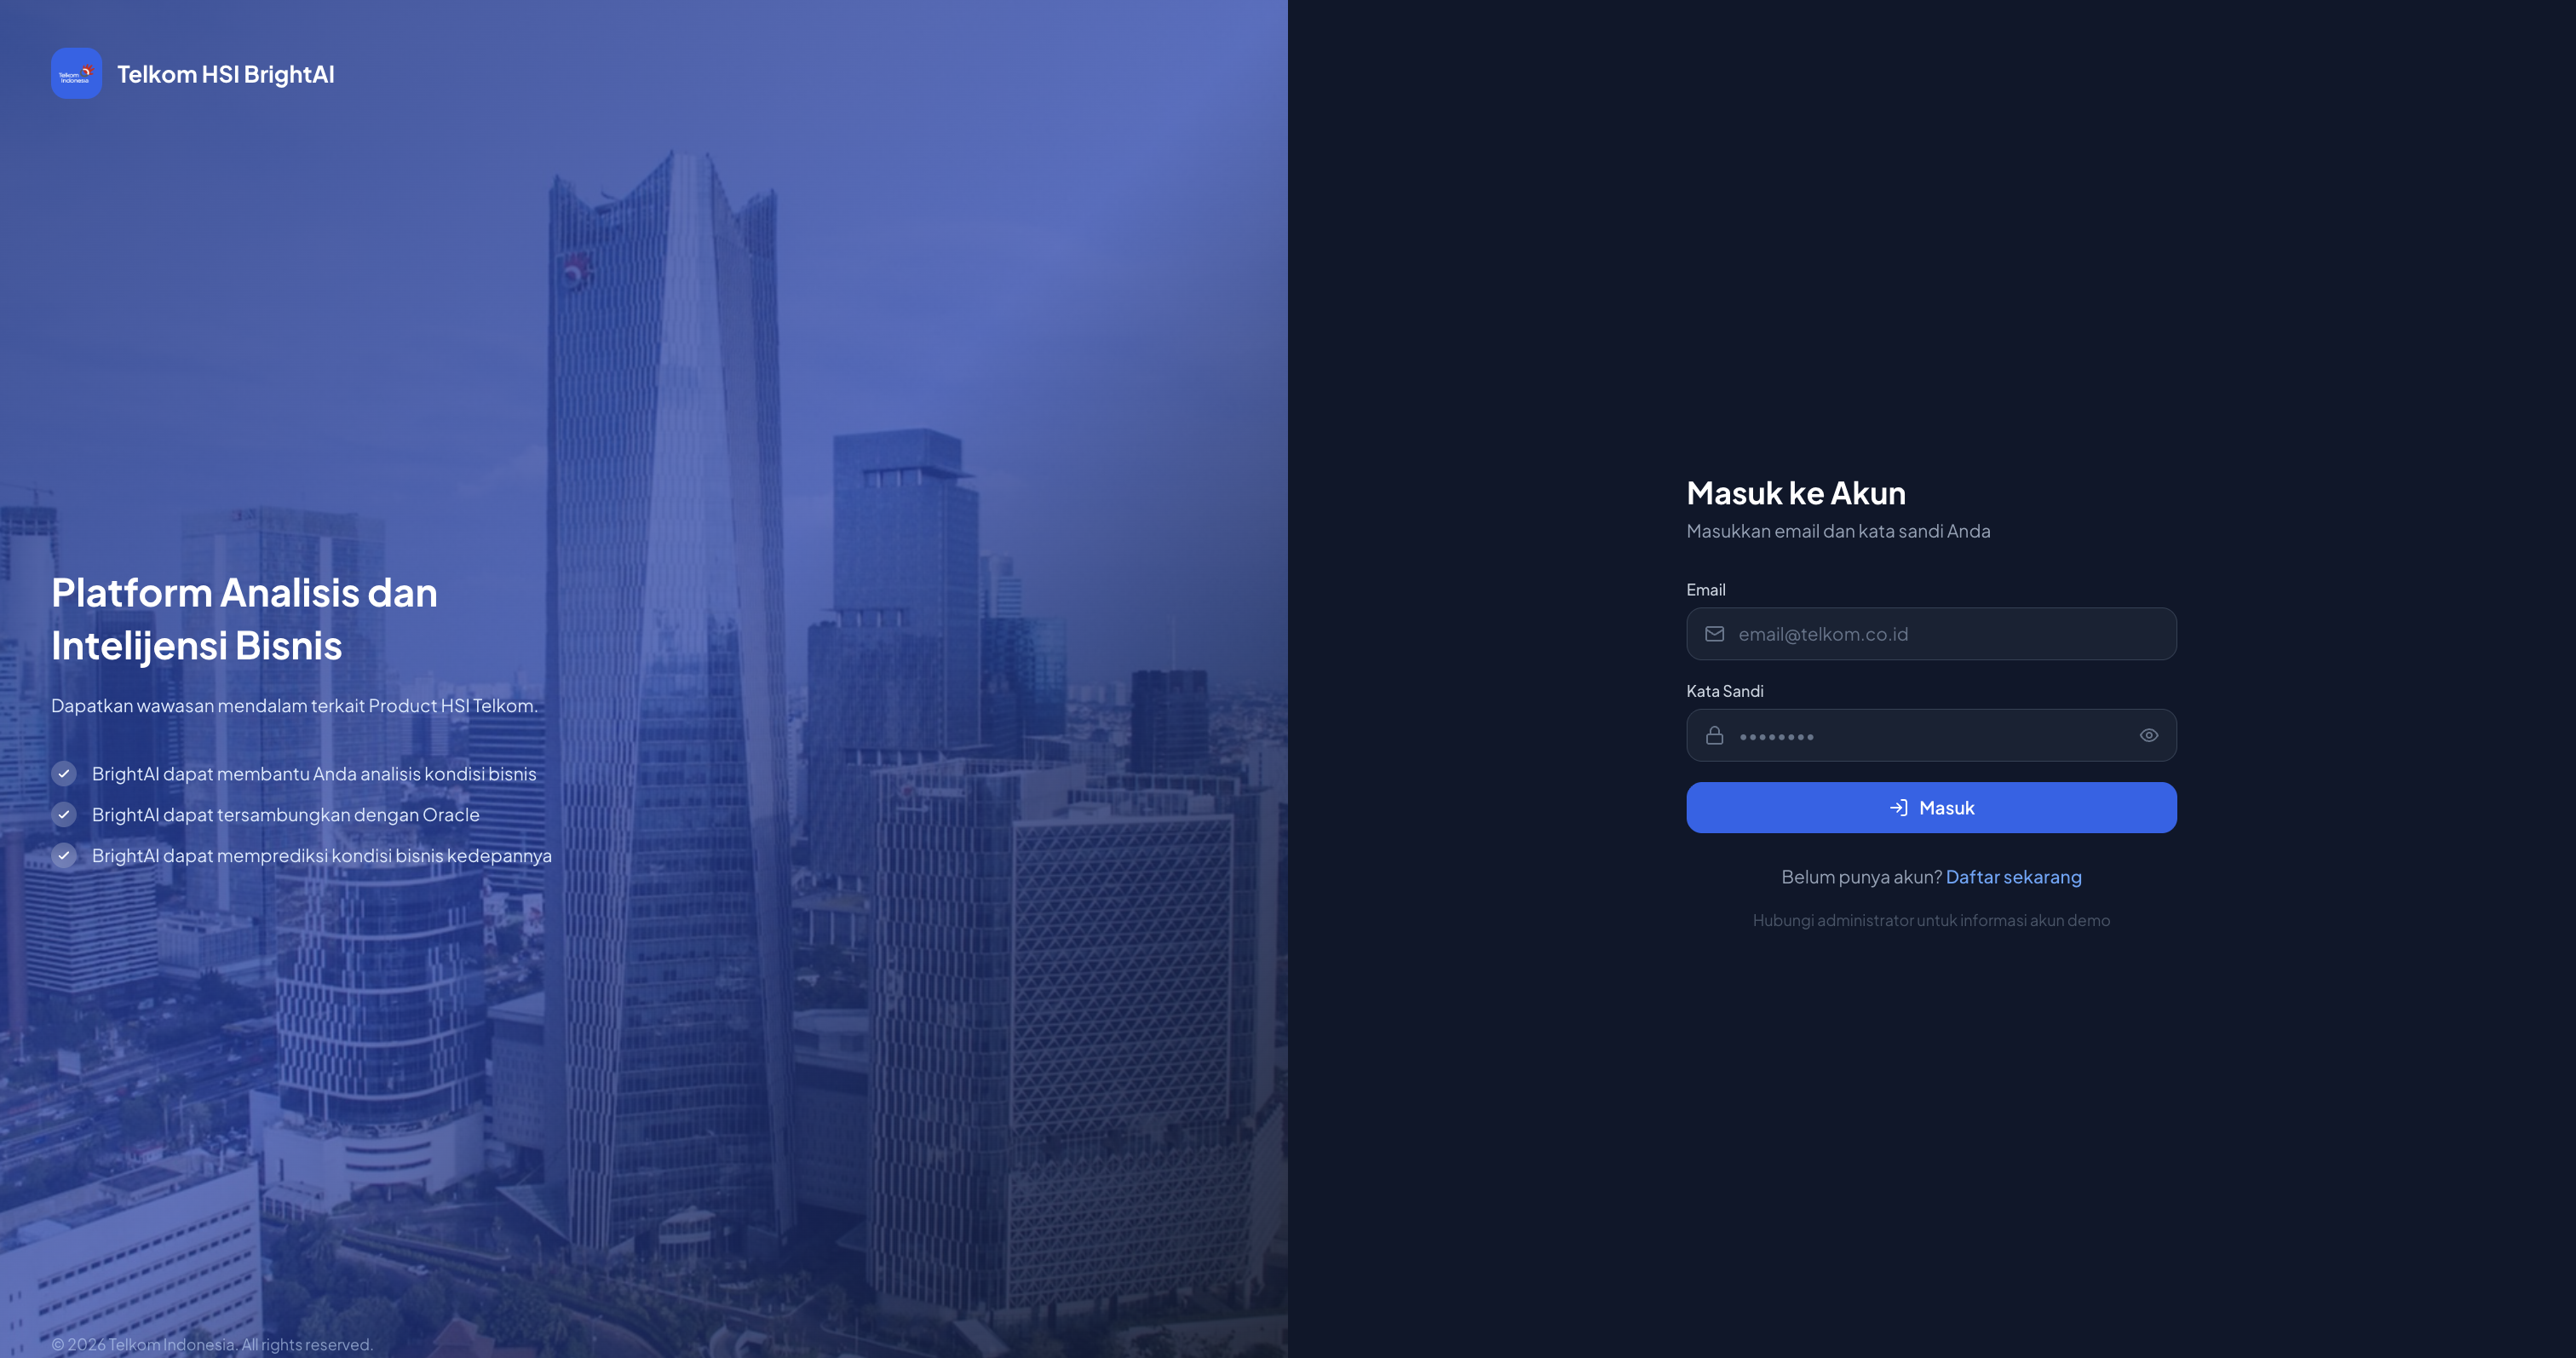
\includegraphics[width=0.85\textwidth]{images/imagemockup1}
\caption{Halaman Masuk (\textit{Login}) Sistem BrightAI}
\label{fig:ui-login}
\end{figure}

\subsubsection{Halaman Registrasi}

Halaman registrasi memungkinkan pengguna internal baru untuk membuat akun pada sistem BrightAI. Formulir registrasi meminta empat isian, yaitu \textit{username}, alamat surel, nama lengkap, dan kata sandi dengan persyaratan minimal enam karakter yang terdiri dari kombinasi huruf besar, huruf kecil, dan angka. Halaman ini dapat diakses melalui tautan ``Daftar sekarang'' pada halaman masuk, dan sebaliknya pengguna yang telah memiliki akun dapat kembali ke halaman masuk melalui tautan ``Masuk''. Gambar~\ref{fig:ui-register} menunjukkan tampilan halaman registrasi.

\begin{figure}[h]
\centering
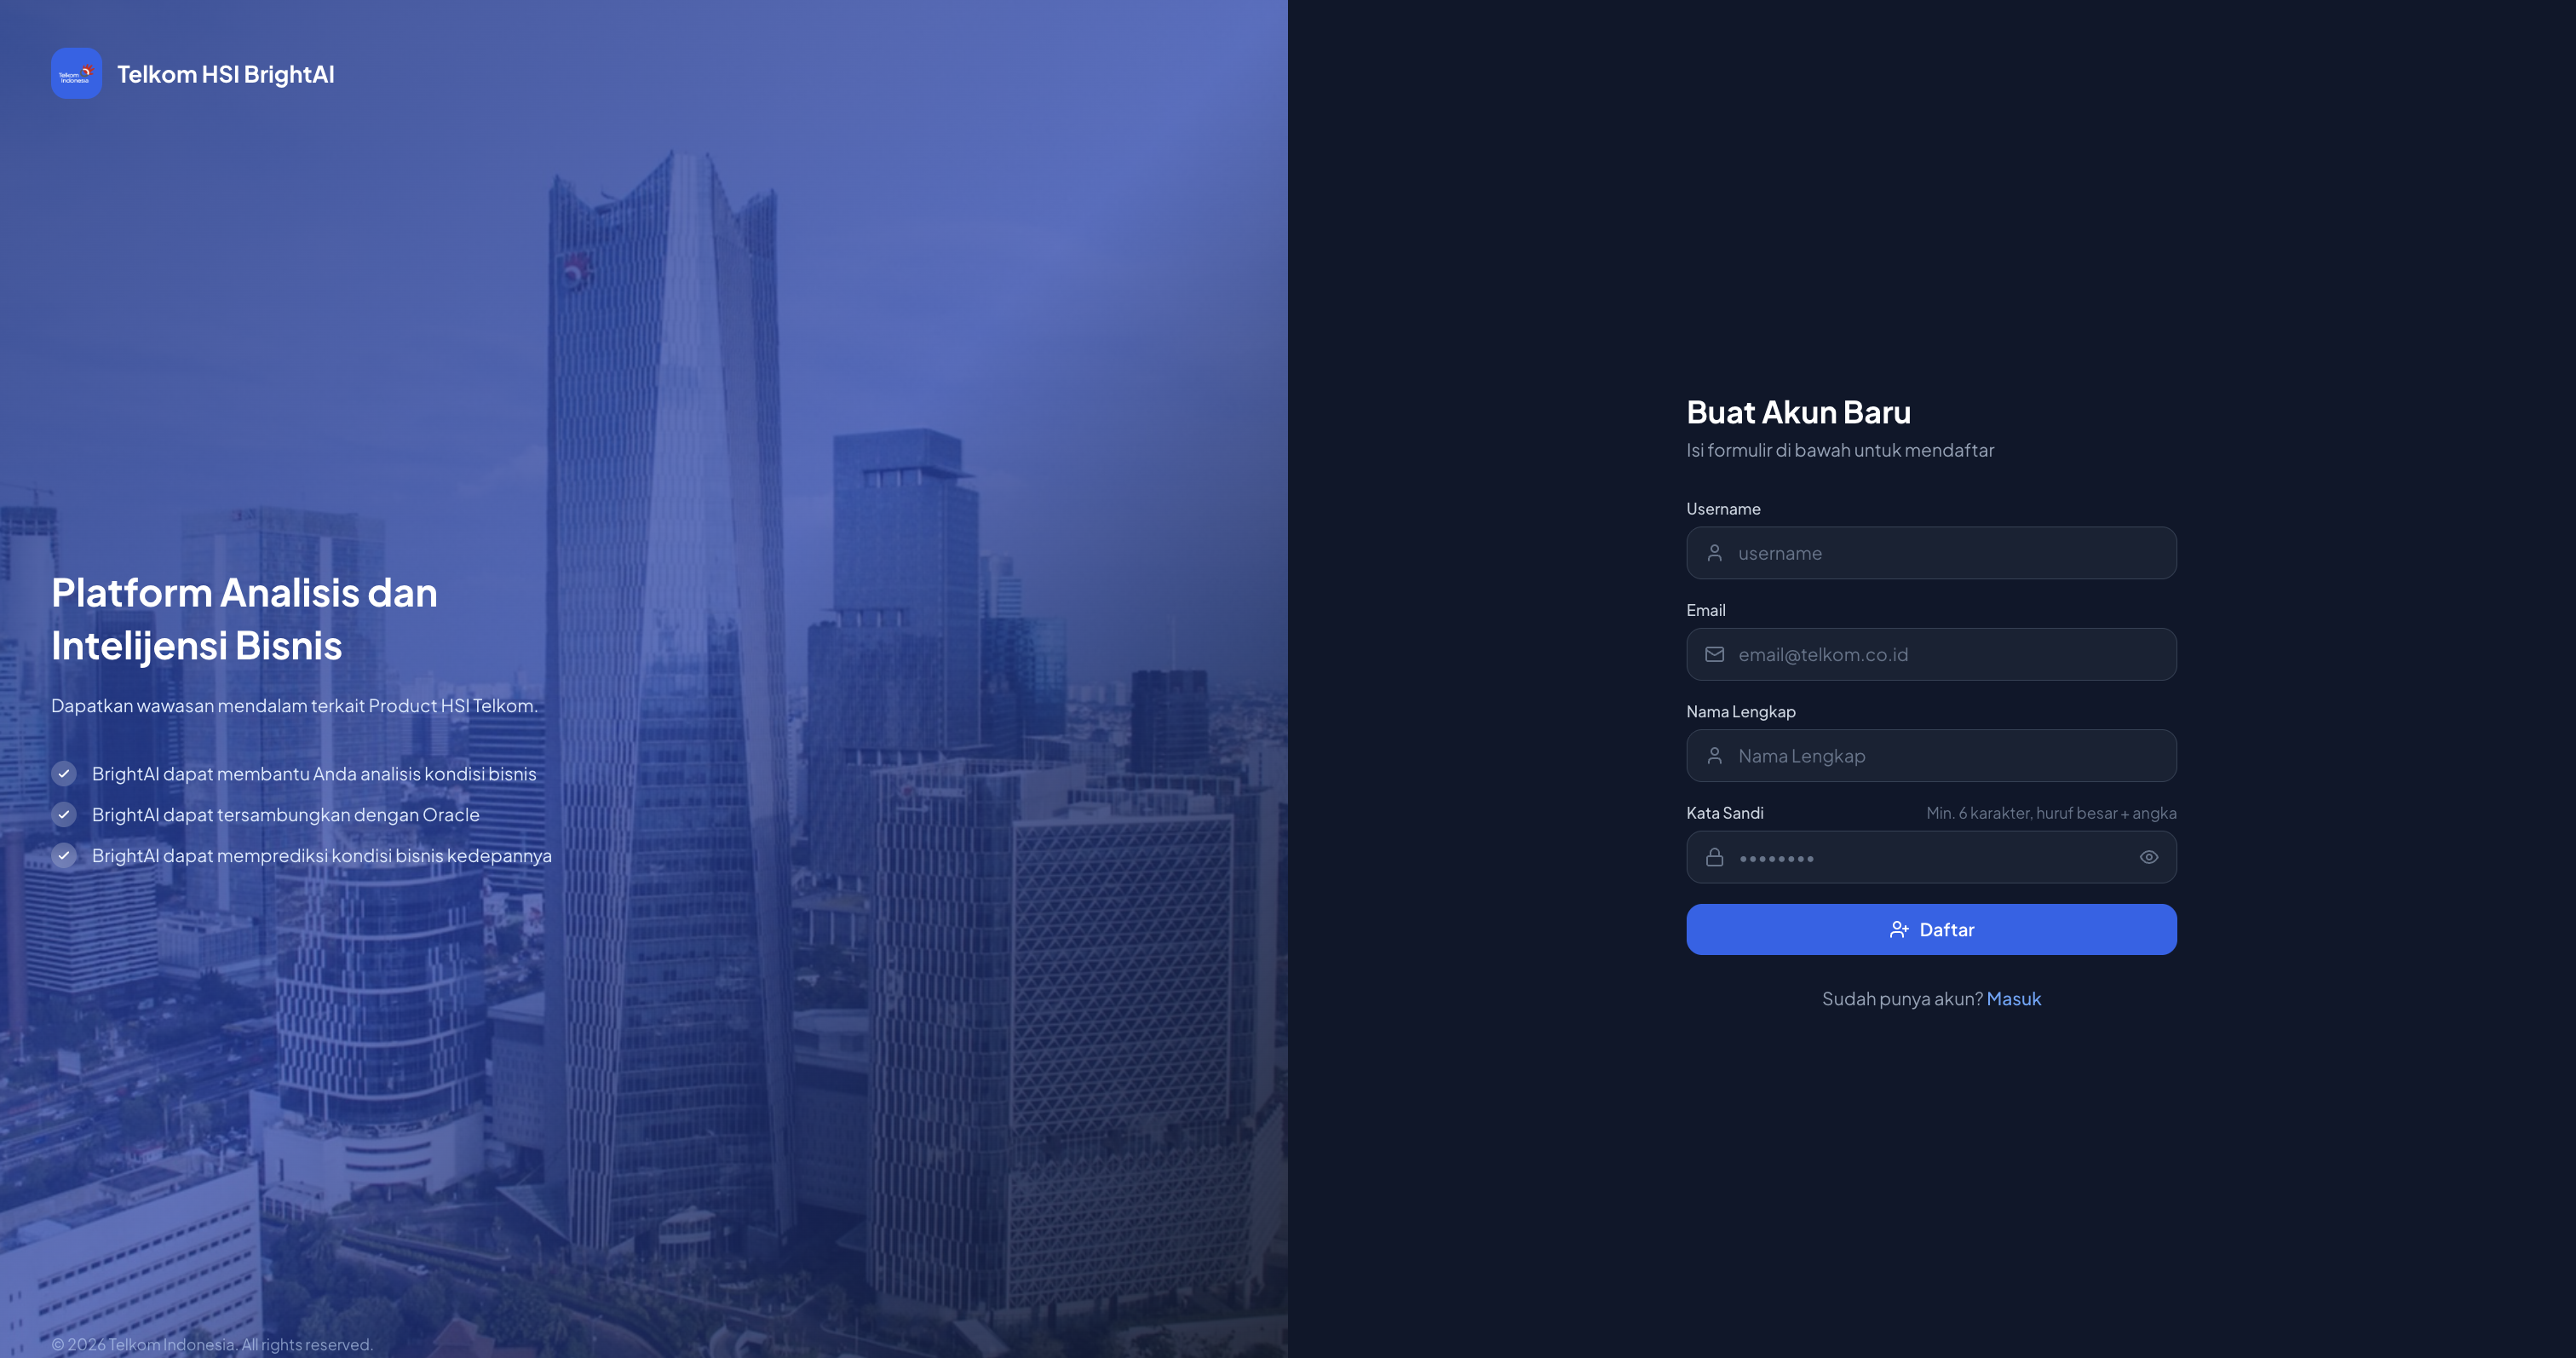
\includegraphics[width=0.85\textwidth]{images/imagemockup2}
\caption{Halaman Registrasi Pengguna Baru}
\label{fig:ui-register}
\end{figure}

\subsubsection{Halaman Utama \textit{Chatbot}}

Halaman utama \textit{chatbot} merupakan antarmuka inti sistem yang terdiri dari tiga area: (1)~bilah navigasi vertikal di sisi kiri yang menyediakan akses ke modul \textit{chatbot}, profil, dan pengaturan; (2)~panel riwayat percakapan yang memungkinkan pengguna mengelola sesi percakapan, termasuk pencarian, penggantian nama, penyematan (\textit{pin}), dan penghapusan sesi; serta (3)~area percakapan utama yang menampilkan pesan pengguna dan respons sistem. Di bagian bawah, alur terpandu (\textit{guided flow}) menyediakan mekanisme interaksi terstruktur melalui pemilihan jenis analisis, kategori domain, dan pertanyaan yang telah dikurasi. Bilah tajuk di bagian atas menampilkan status koneksi server, pengalih tema, dan informasi pengguna. Gambar~\ref{fig:ui-chat} menunjukkan tampilan halaman utama \textit{chatbot}.

\begin{figure}[h]
\centering
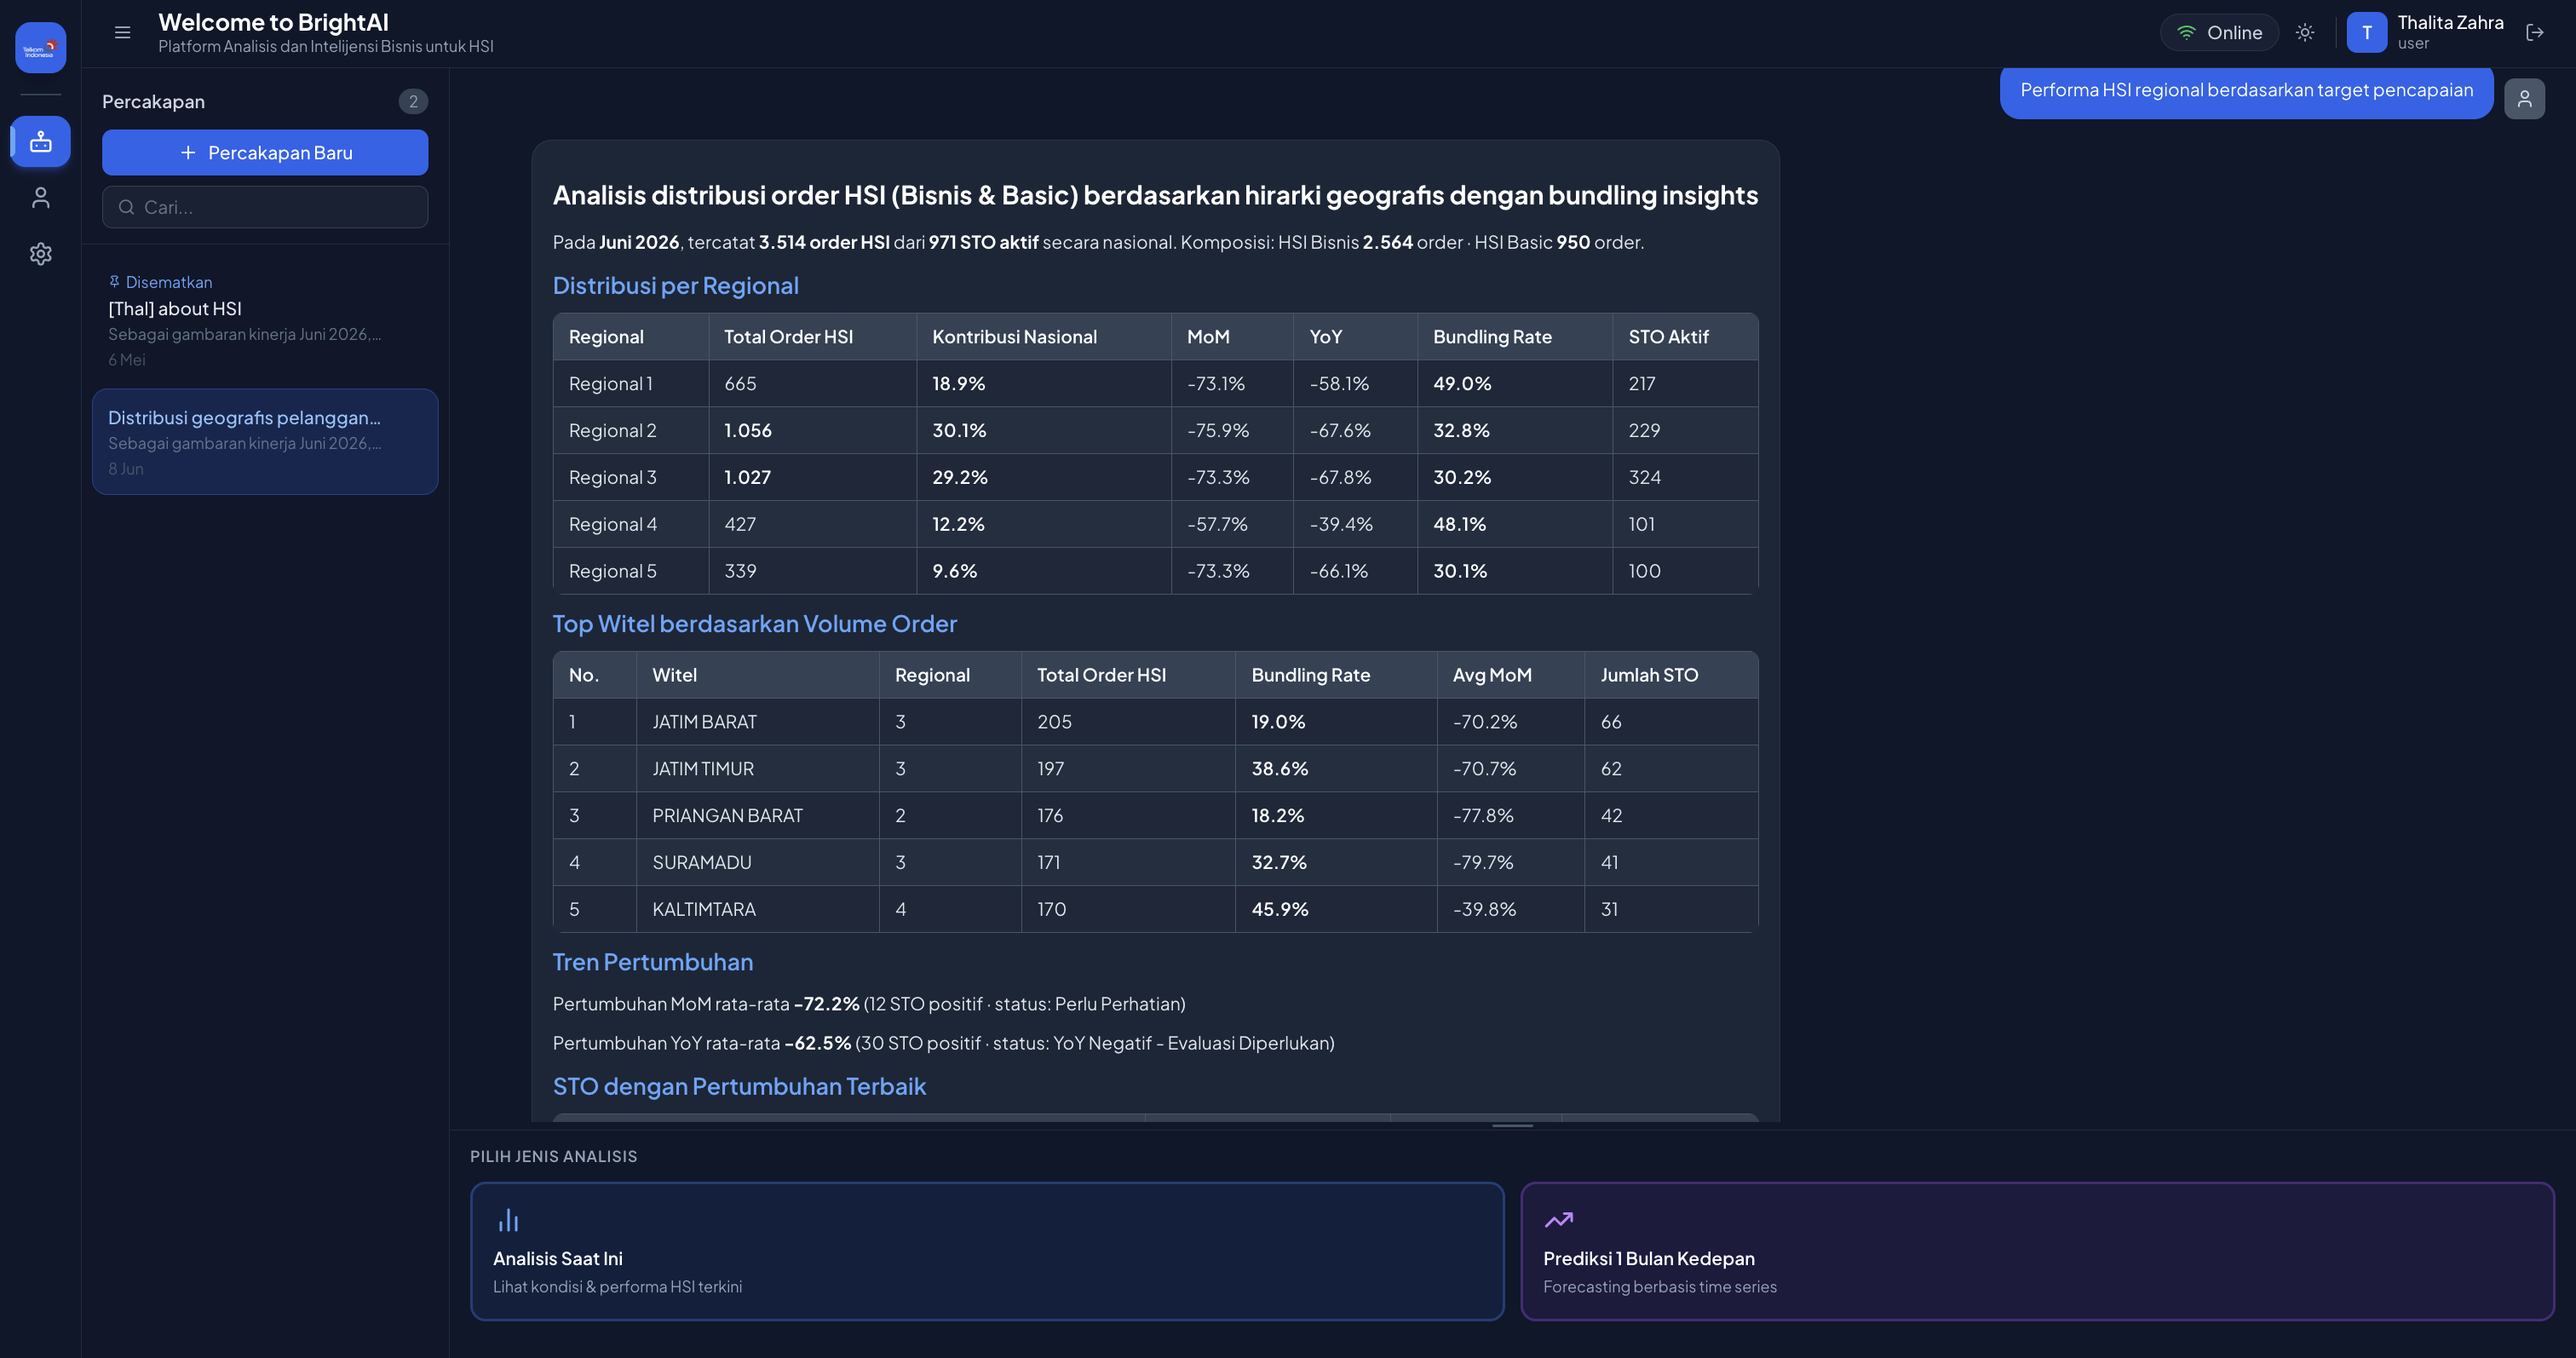
\includegraphics[width=0.85\textwidth]{images/imagemockup3}
\caption{Halaman Utama \textit{Chatbot} BrightAI}
\label{fig:ui-chat}
\end{figure}

\subsubsection{Halaman Profil}

Halaman profil menampilkan informasi akun pengguna yang sedang masuk, meliputi nama lengkap, \textit{username}, alamat surel, dan peran (\textit{role}) dalam sistem. Halaman ini dapat diakses melalui ikon pengguna pada bilah navigasi vertikal. Gambar~\ref{fig:ui-profile} menunjukkan tampilan halaman profil.

\begin{figure}[h]
\centering
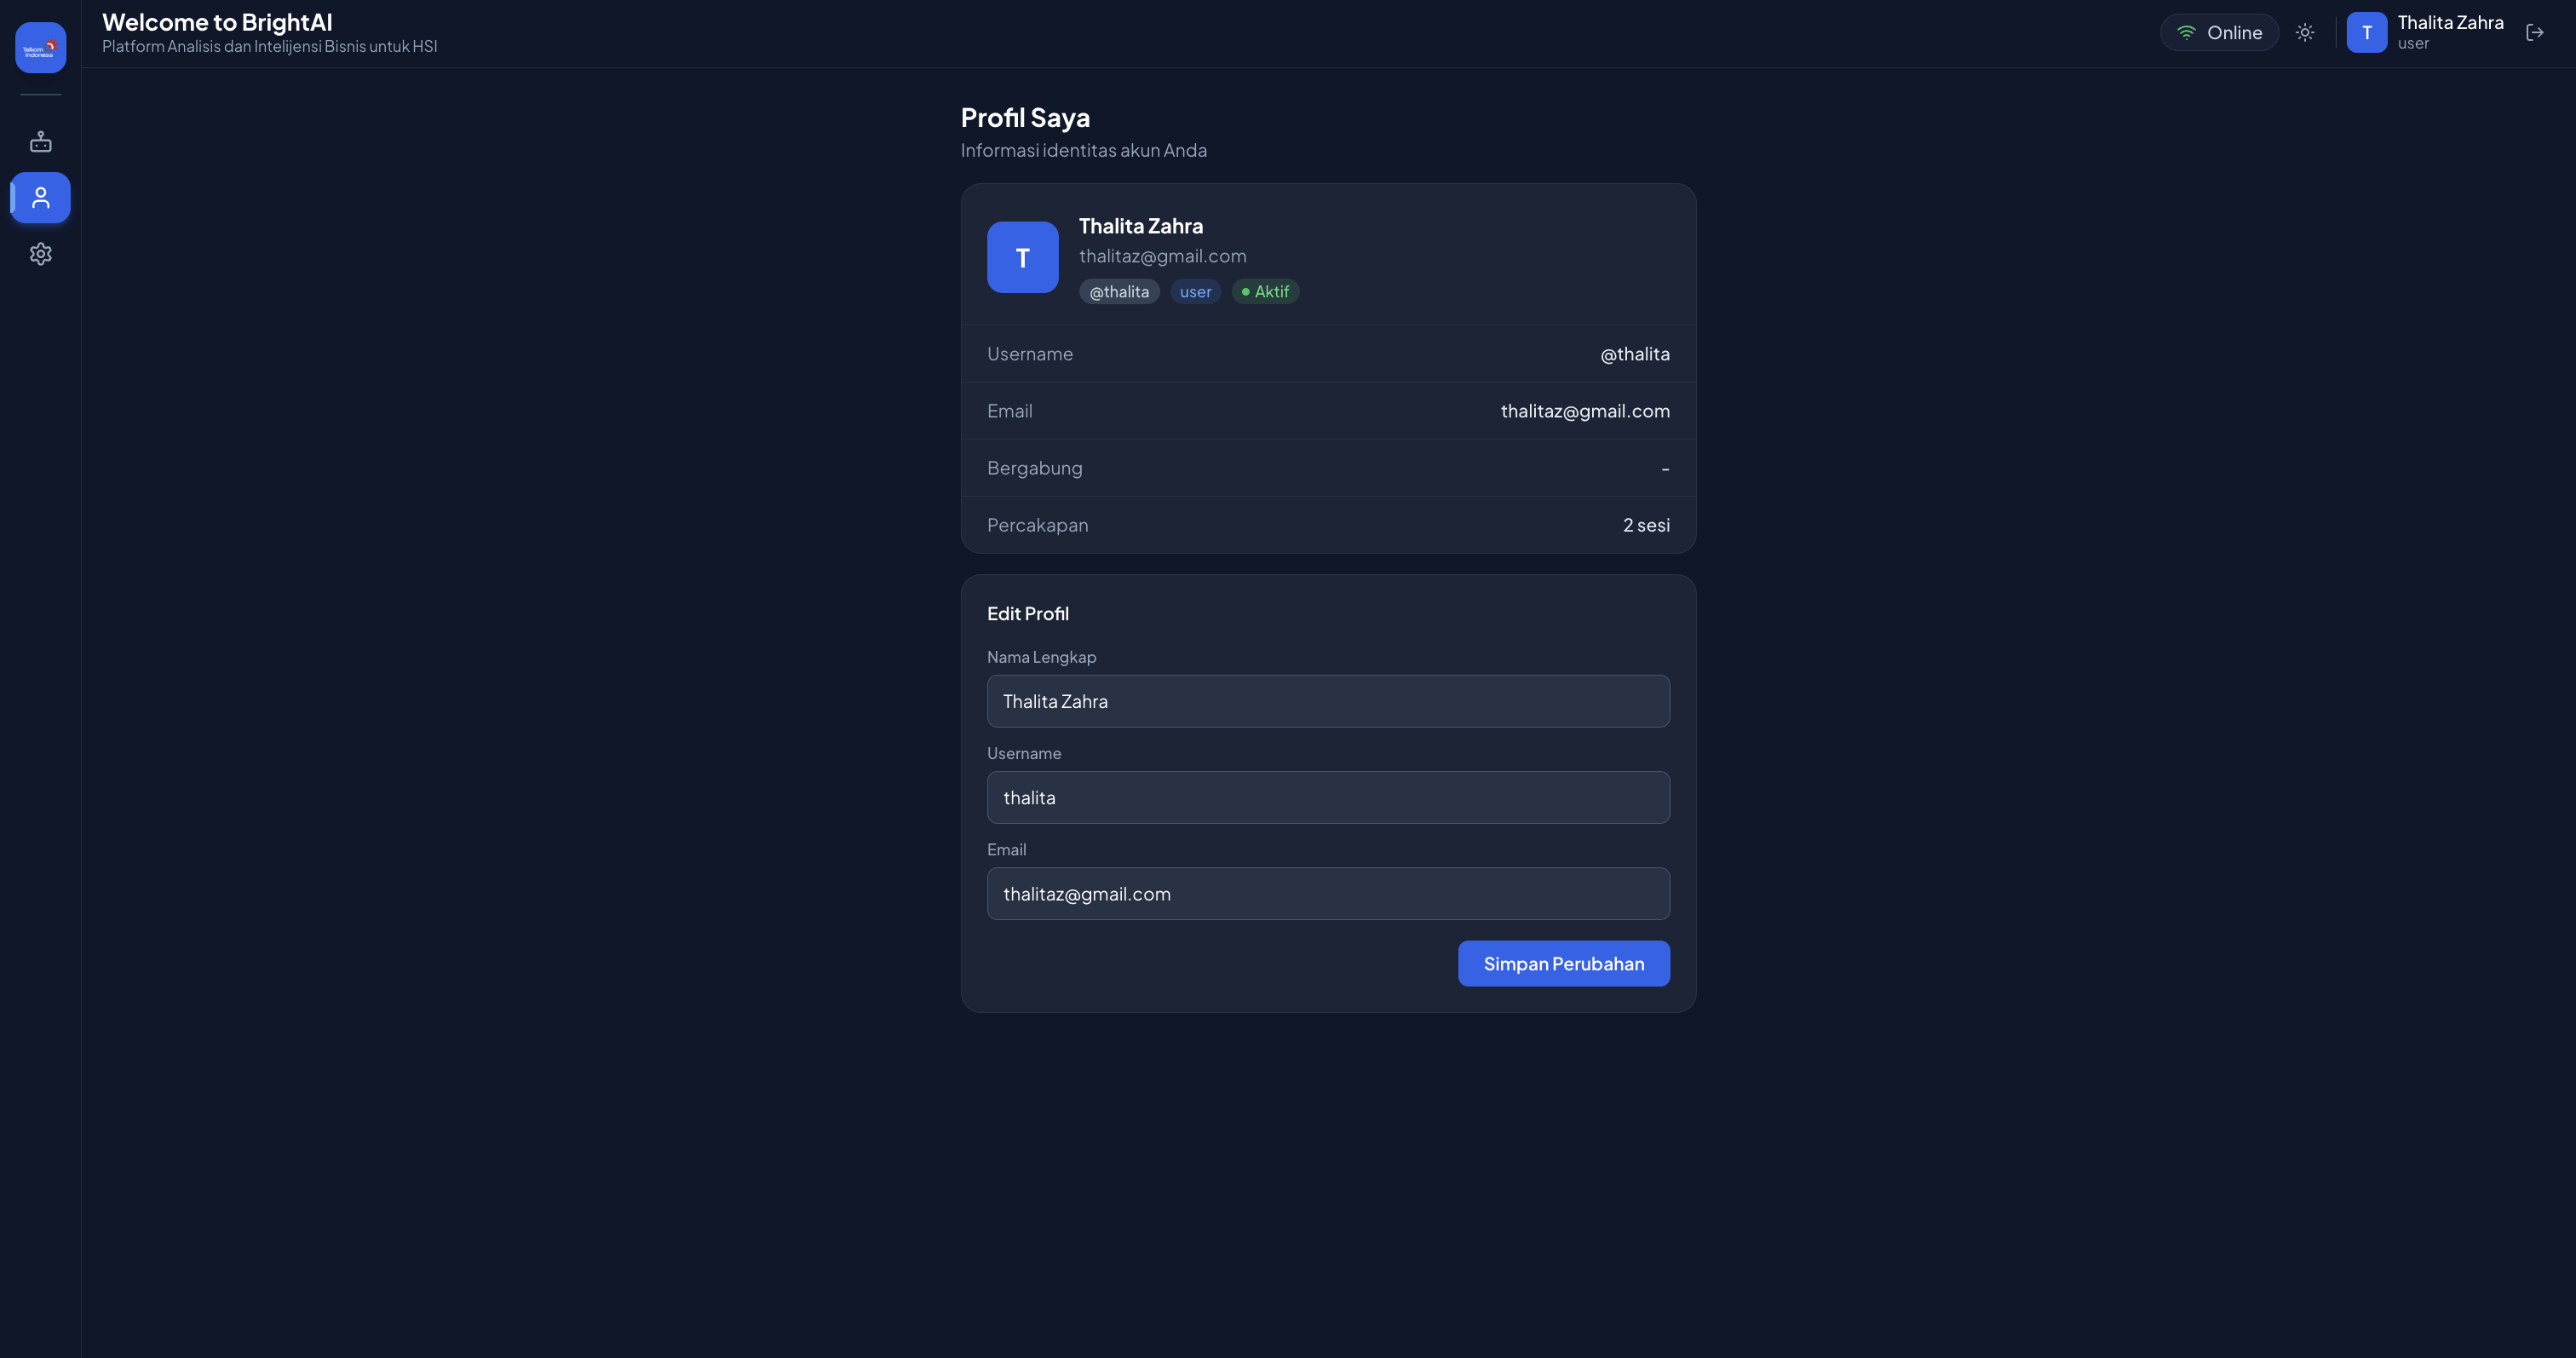
\includegraphics[width=0.85\textwidth]{images/imagemockup4}
\caption{Halaman Profil Pengguna}
\label{fig:ui-profile}
\end{figure}

\subsubsection{Halaman Pengaturan}

Halaman pengaturan menyediakan opsi konfigurasi antarmuka bagi pengguna, termasuk pengalihan tema tampilan dan preferensi notifikasi. Halaman ini dapat diakses melalui ikon pengaturan pada bilah navigasi vertikal. Gambar~\ref{fig:ui-settings} menunjukkan tampilan halaman pengaturan.

\begin{figure}[h]
\centering
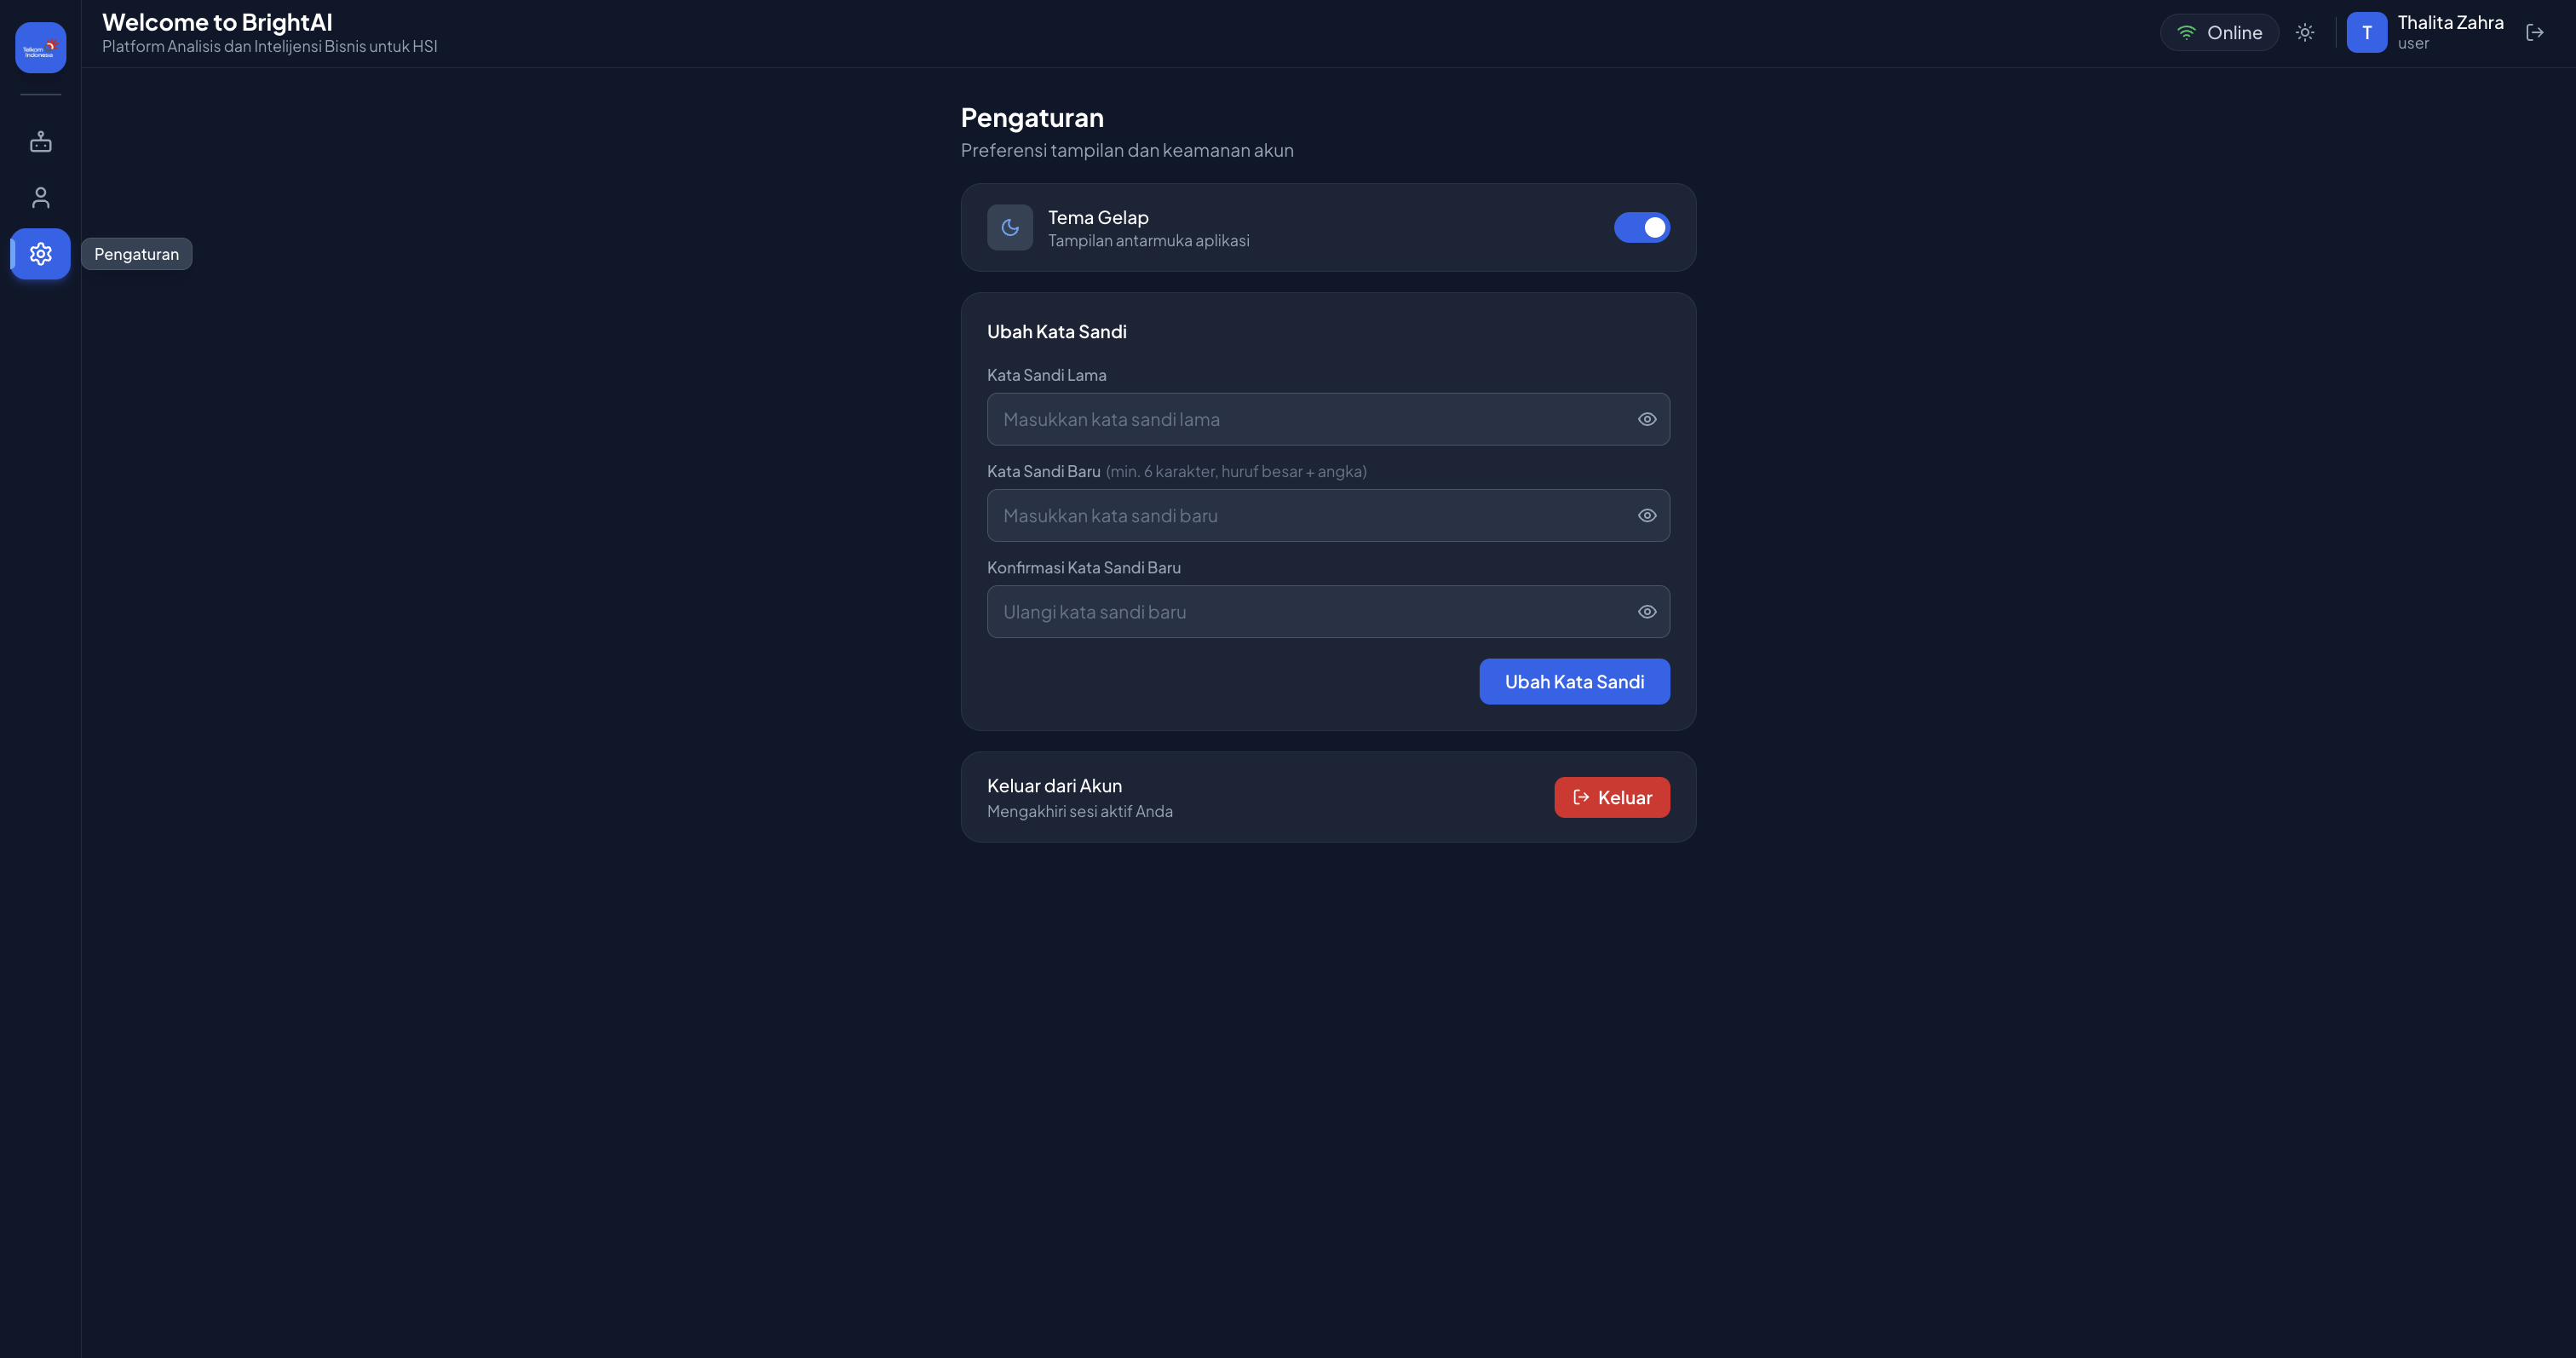
\includegraphics[width=0.85\textwidth]{images/imagemockup5}
\caption{Halaman Pengaturan Sistem}
\label{fig:ui-settings}
\end{figure}

\subsubsection{Tampilan Tema Terang (\textit{Light Mode})}

Sistem mendukung dua tema tampilan, yaitu tema gelap (\textit{dark mode}) sebagai tema bawaan dan tema terang (\textit{light mode}). Pengguna dapat beralih antara kedua tema melalui tombol pengalih pada bilah tajuk. Seluruh komponen antarmuka, termasuk area percakapan, panel riwayat, dan alur terpandu, menyesuaikan skema warna secara konsisten sesuai tema yang dipilih. Gambar~\ref{fig:ui-light} menunjukkan tampilan sistem dalam tema terang.

\begin{figure}[h]
\centering
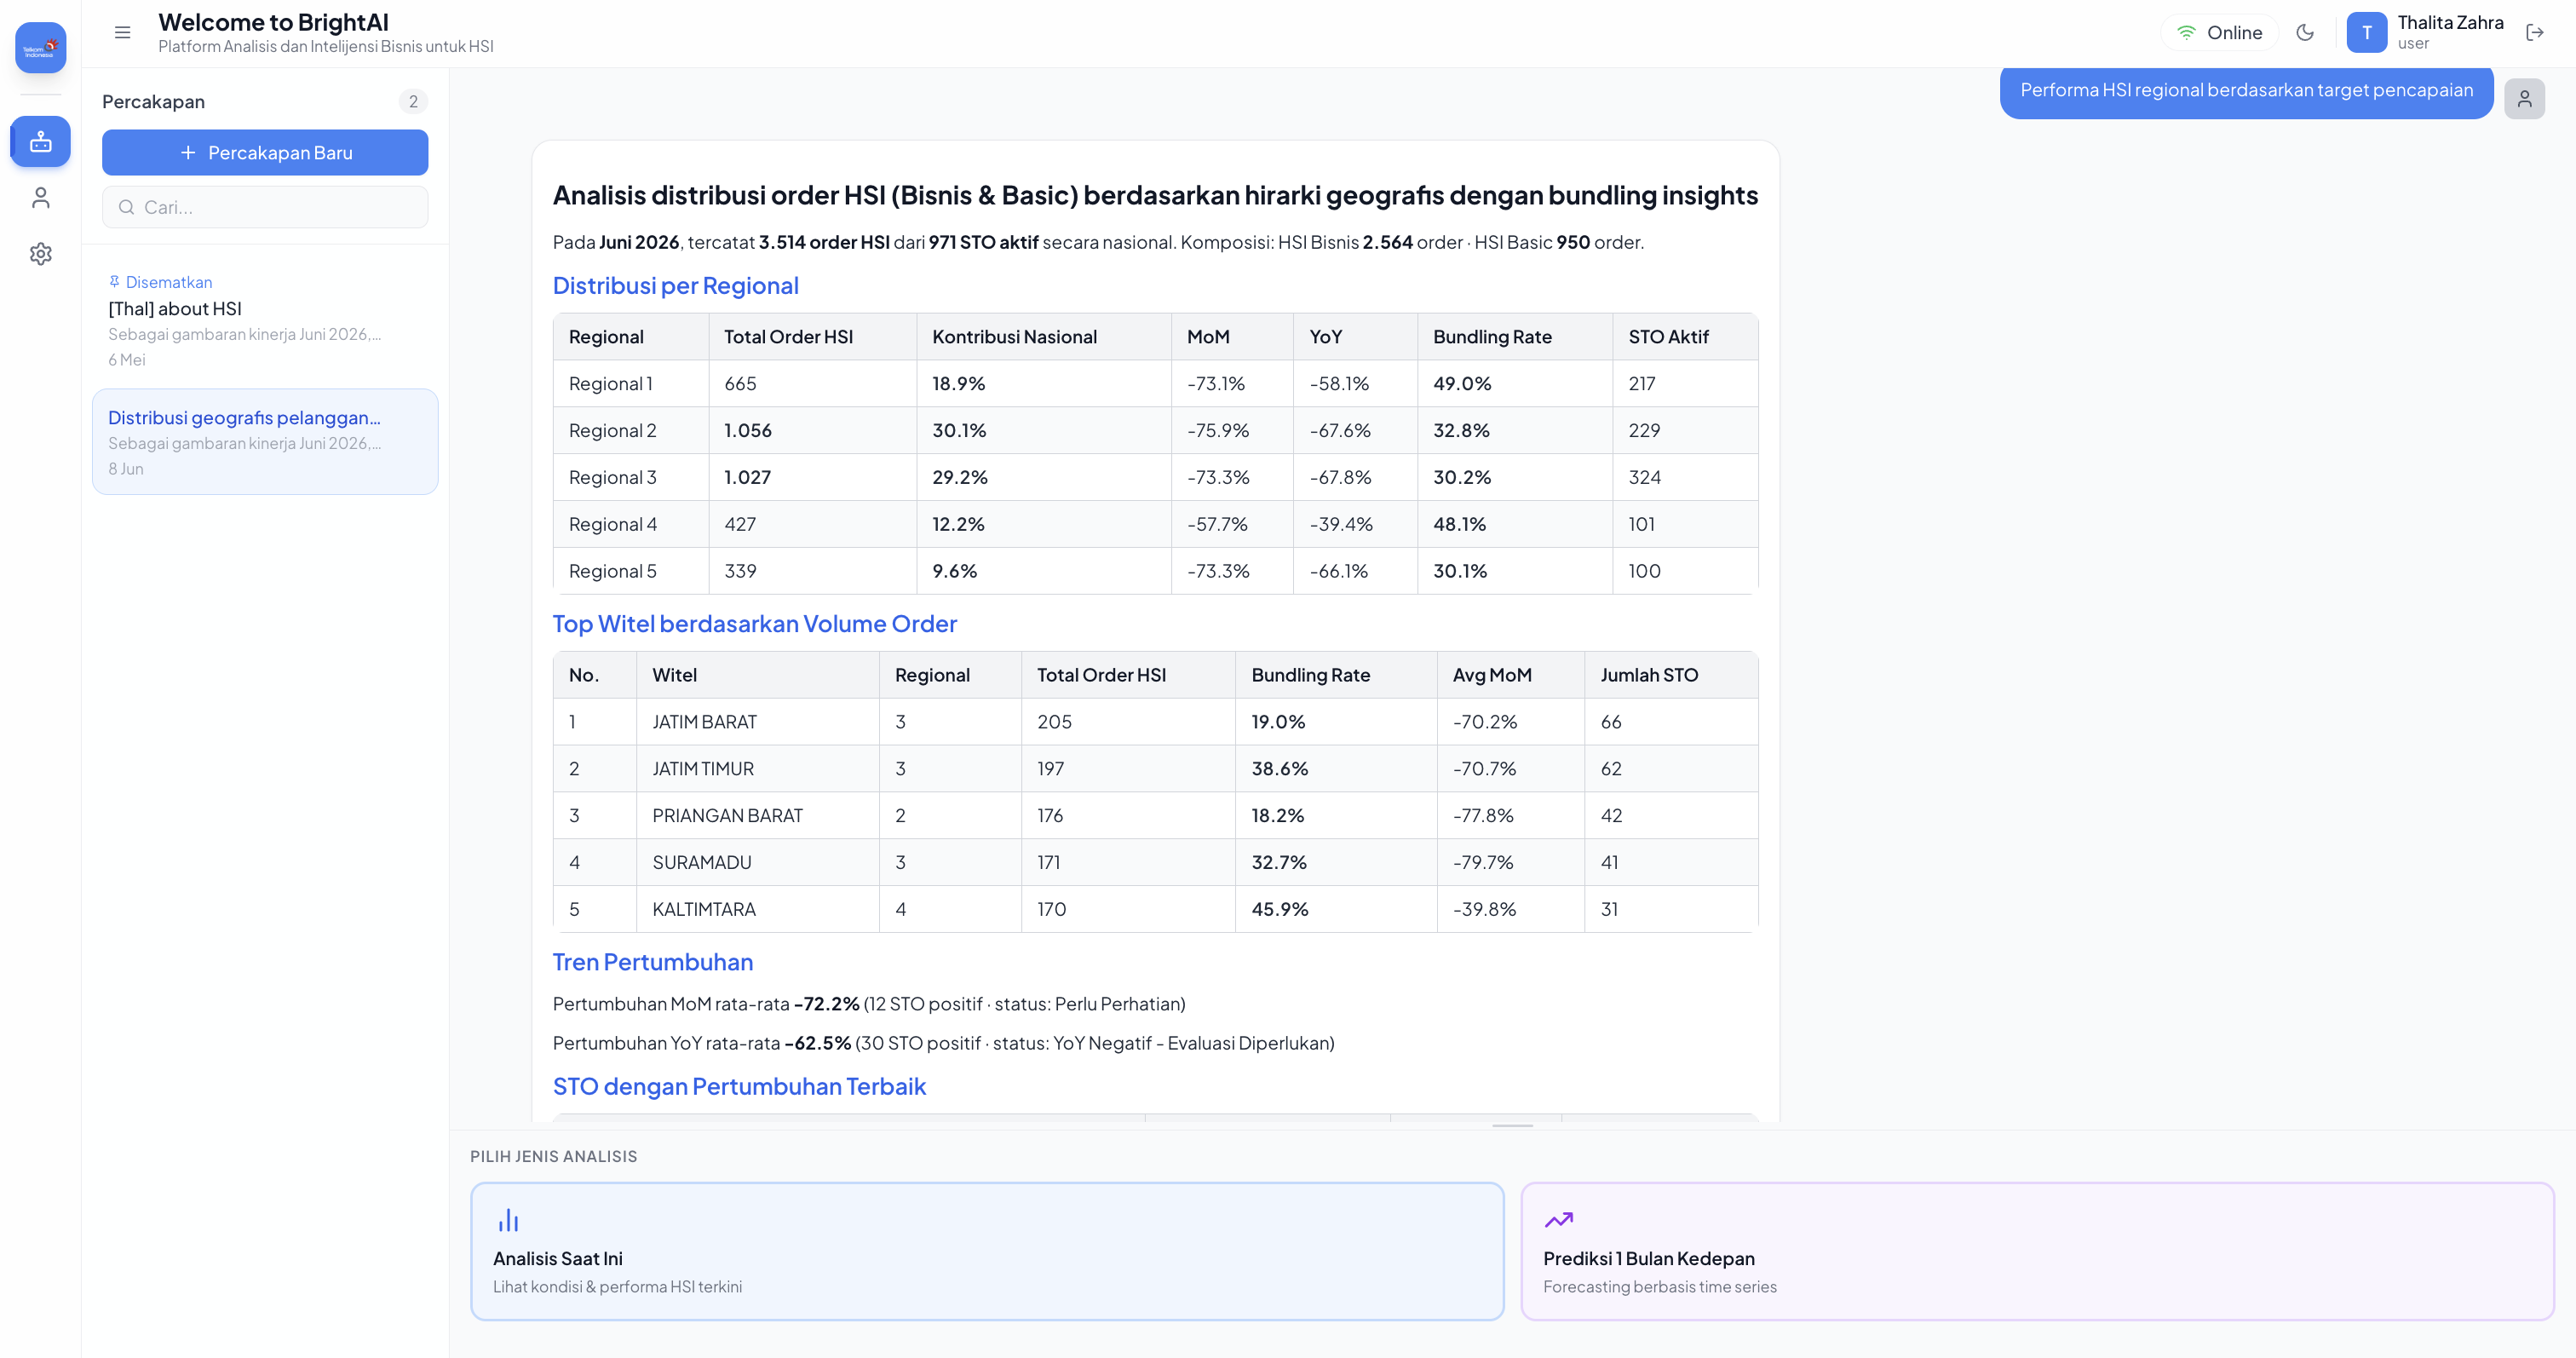
\includegraphics[width=0.85\textwidth]{images/imagemockup6}
\caption{Tampilan Antarmuka \textit{Chatbot} dalam Tema Terang (\textit{Light Mode})}
\label{fig:ui-light}
\end{figure}

\subsubsection{Detail Respons \textit{Rule-Based Query}}

Ketika pengguna mengajukan pertanyaan analitik melalui antarmuka percakapan, sistem mencocokkan kueri tersebut dengan salah satu dari 38 aturan bisnis yang tersedia, mengeksekusi kueri SQL terhadap \textit{Enterprise Data Warehouse}, dan menghasilkan respons naratif dalam bahasa Indonesia menggunakan modul NLG berbasis templat. Respons ditampilkan dalam format \textit{Markdown} yang mencakup judul analisis, tabel data dengan angka terformat sesuai konvensi Indonesia, poin-poin wawasan bisnis, serta metadata sumber data dan waktu pemrosesan. Gambar~\ref{fig:ui-rulebased} menunjukkan contoh respons sistem terhadap pertanyaan analitik berbasis aturan.

\begin{figure}[h]
\centering
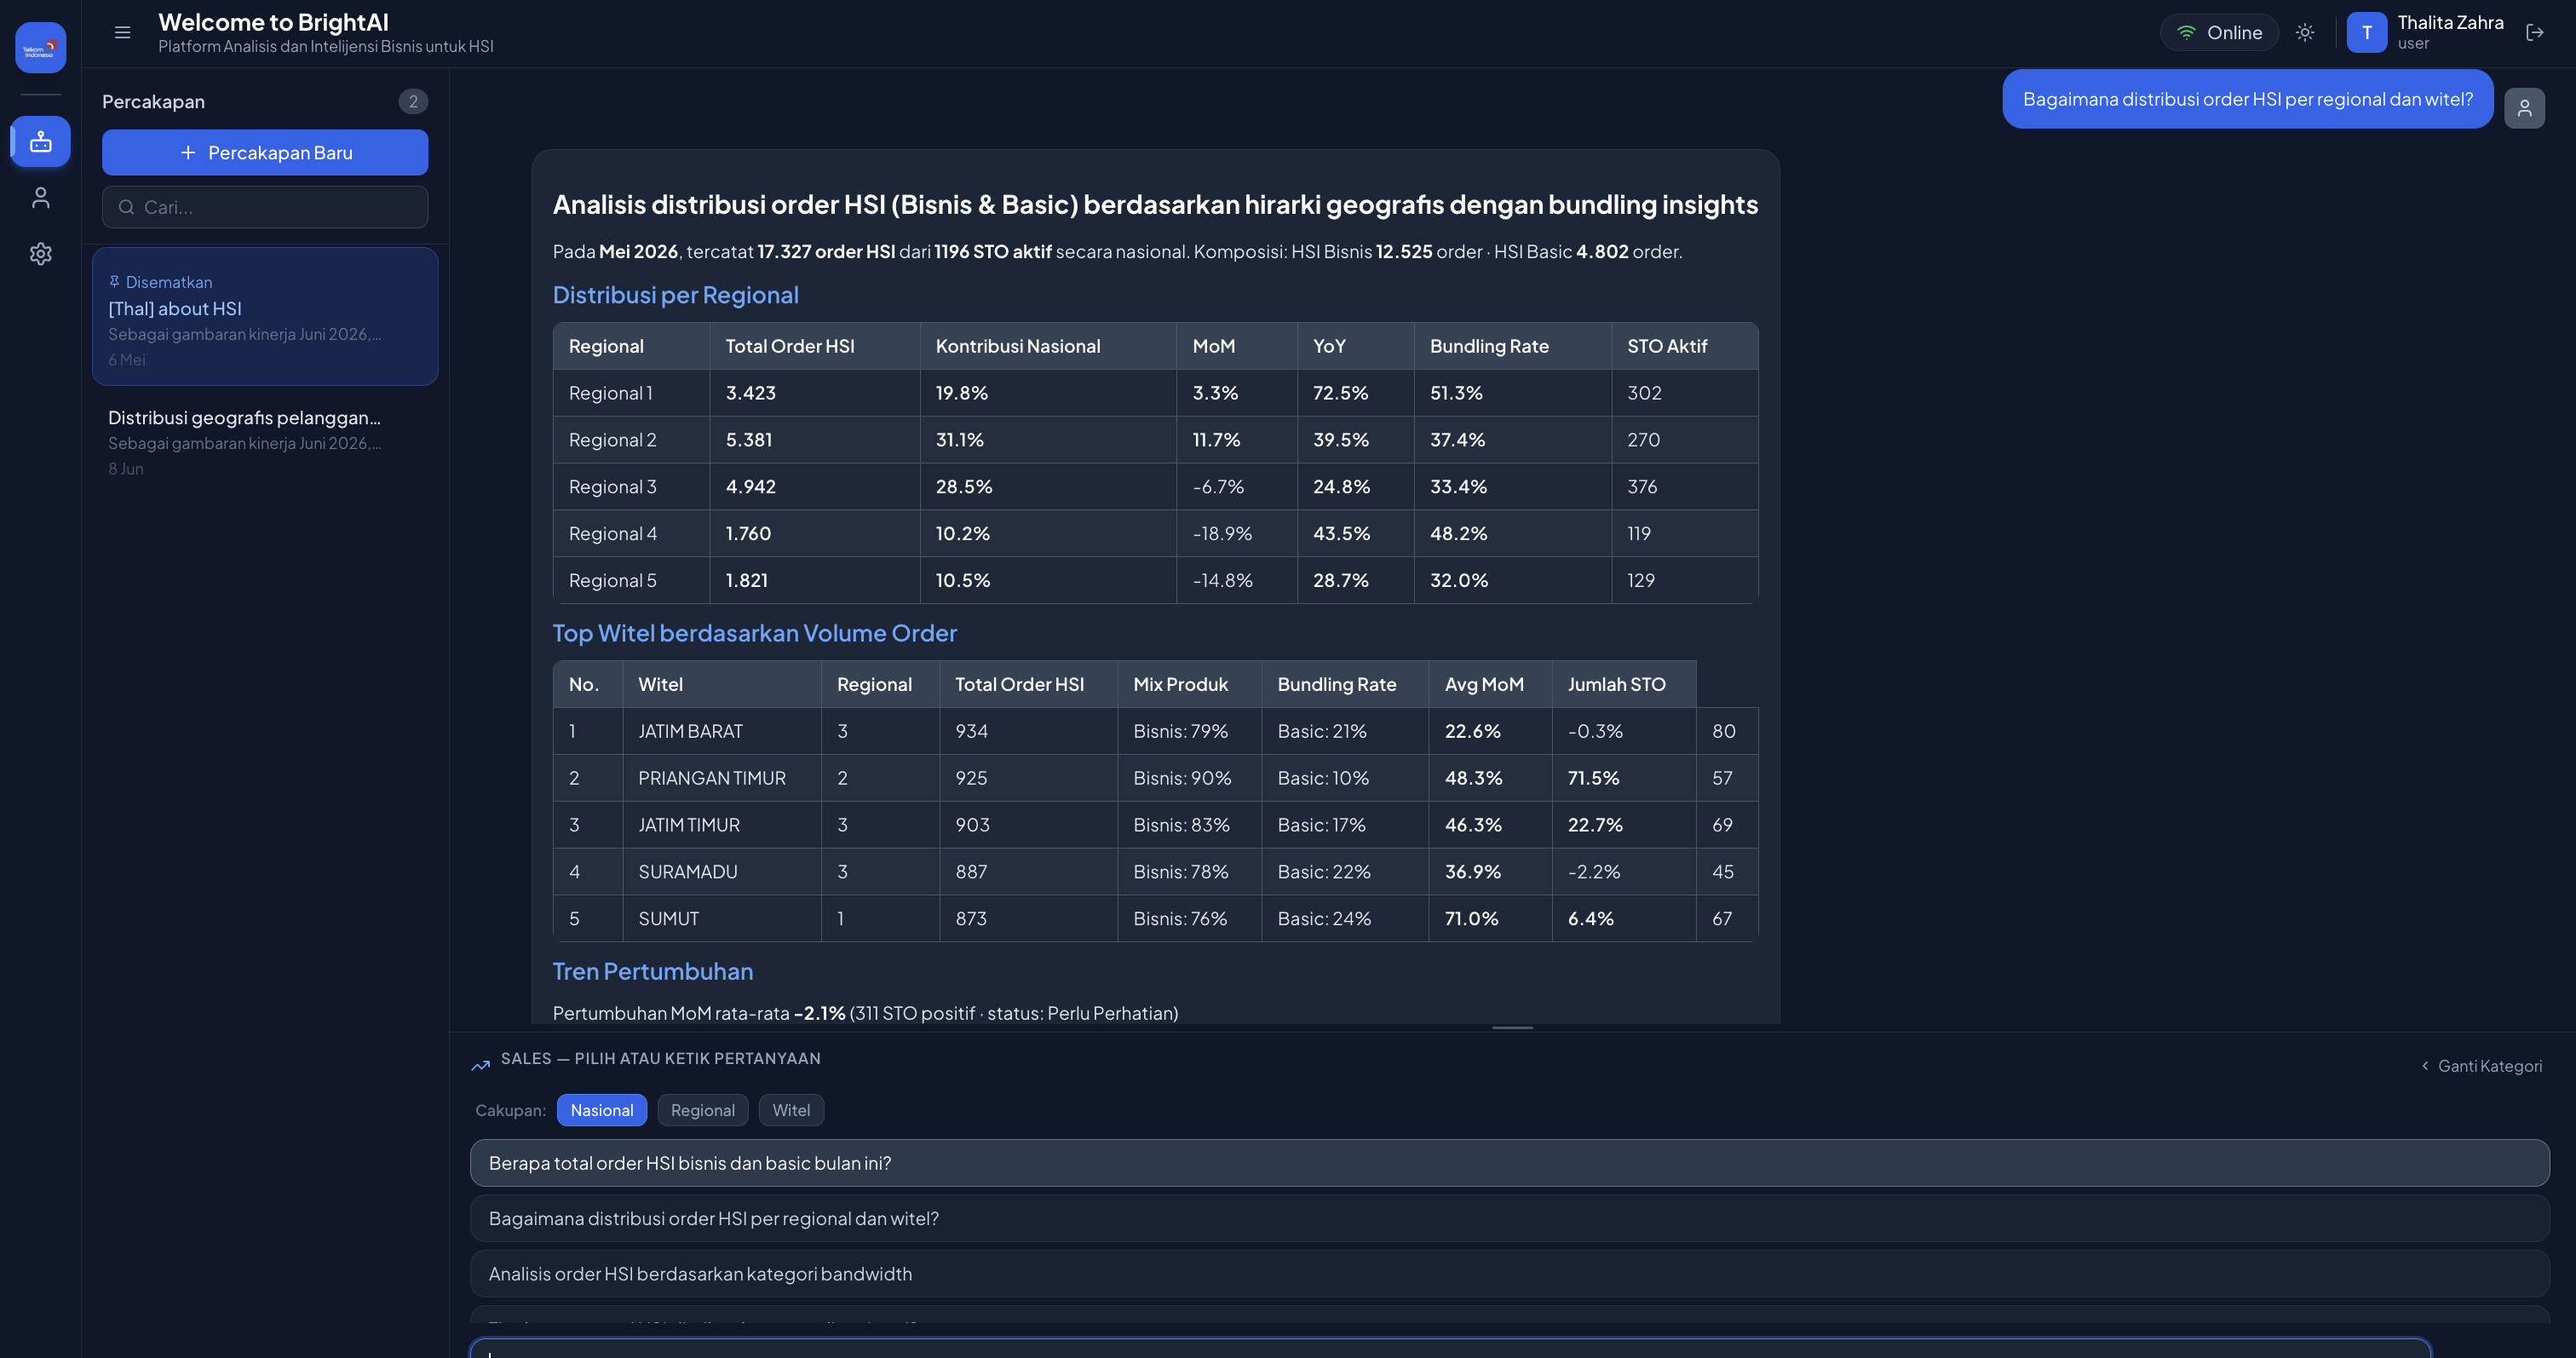
\includegraphics[width=0.85\textwidth]{images/imagemockup7}
\caption{Contoh Respons \textit{Rule-Based Query} dengan Narasi NLG dan Tabel Data}
\label{fig:ui-rulebased}
\end{figure}

\subsubsection{Detail Respons Peramalan Deret Waktu}

Fitur peramalan dapat diakses melalui panel peramalan pada alur terpandu, di mana pengguna memilih metrik yang hendak diramalkan, jenis model (GRU, LSTM, ARIMA, atau \textit{Prophet}), serta cakupan wilayah (nasional, regional, atau \textit{witel}). Hasil peramalan ditampilkan dalam format naratif yang mencakup nilai prediksi untuk periode berikutnya, perbandingan terhadap nilai aktual terakhir, serta metrik evaluasi model (MAE, RMSE, sMAPE, \textit{Skill Score}). Panel ini merupakan realisasi langsung dari tujuan integrasi dan pembandingan model peramalan deret waktu ke dalam antarmuka \textit{chatbot}. Gambar~\ref{fig:ui-forecast} menunjukkan contoh hasil peramalan.

\begin{figure}[h]
\centering
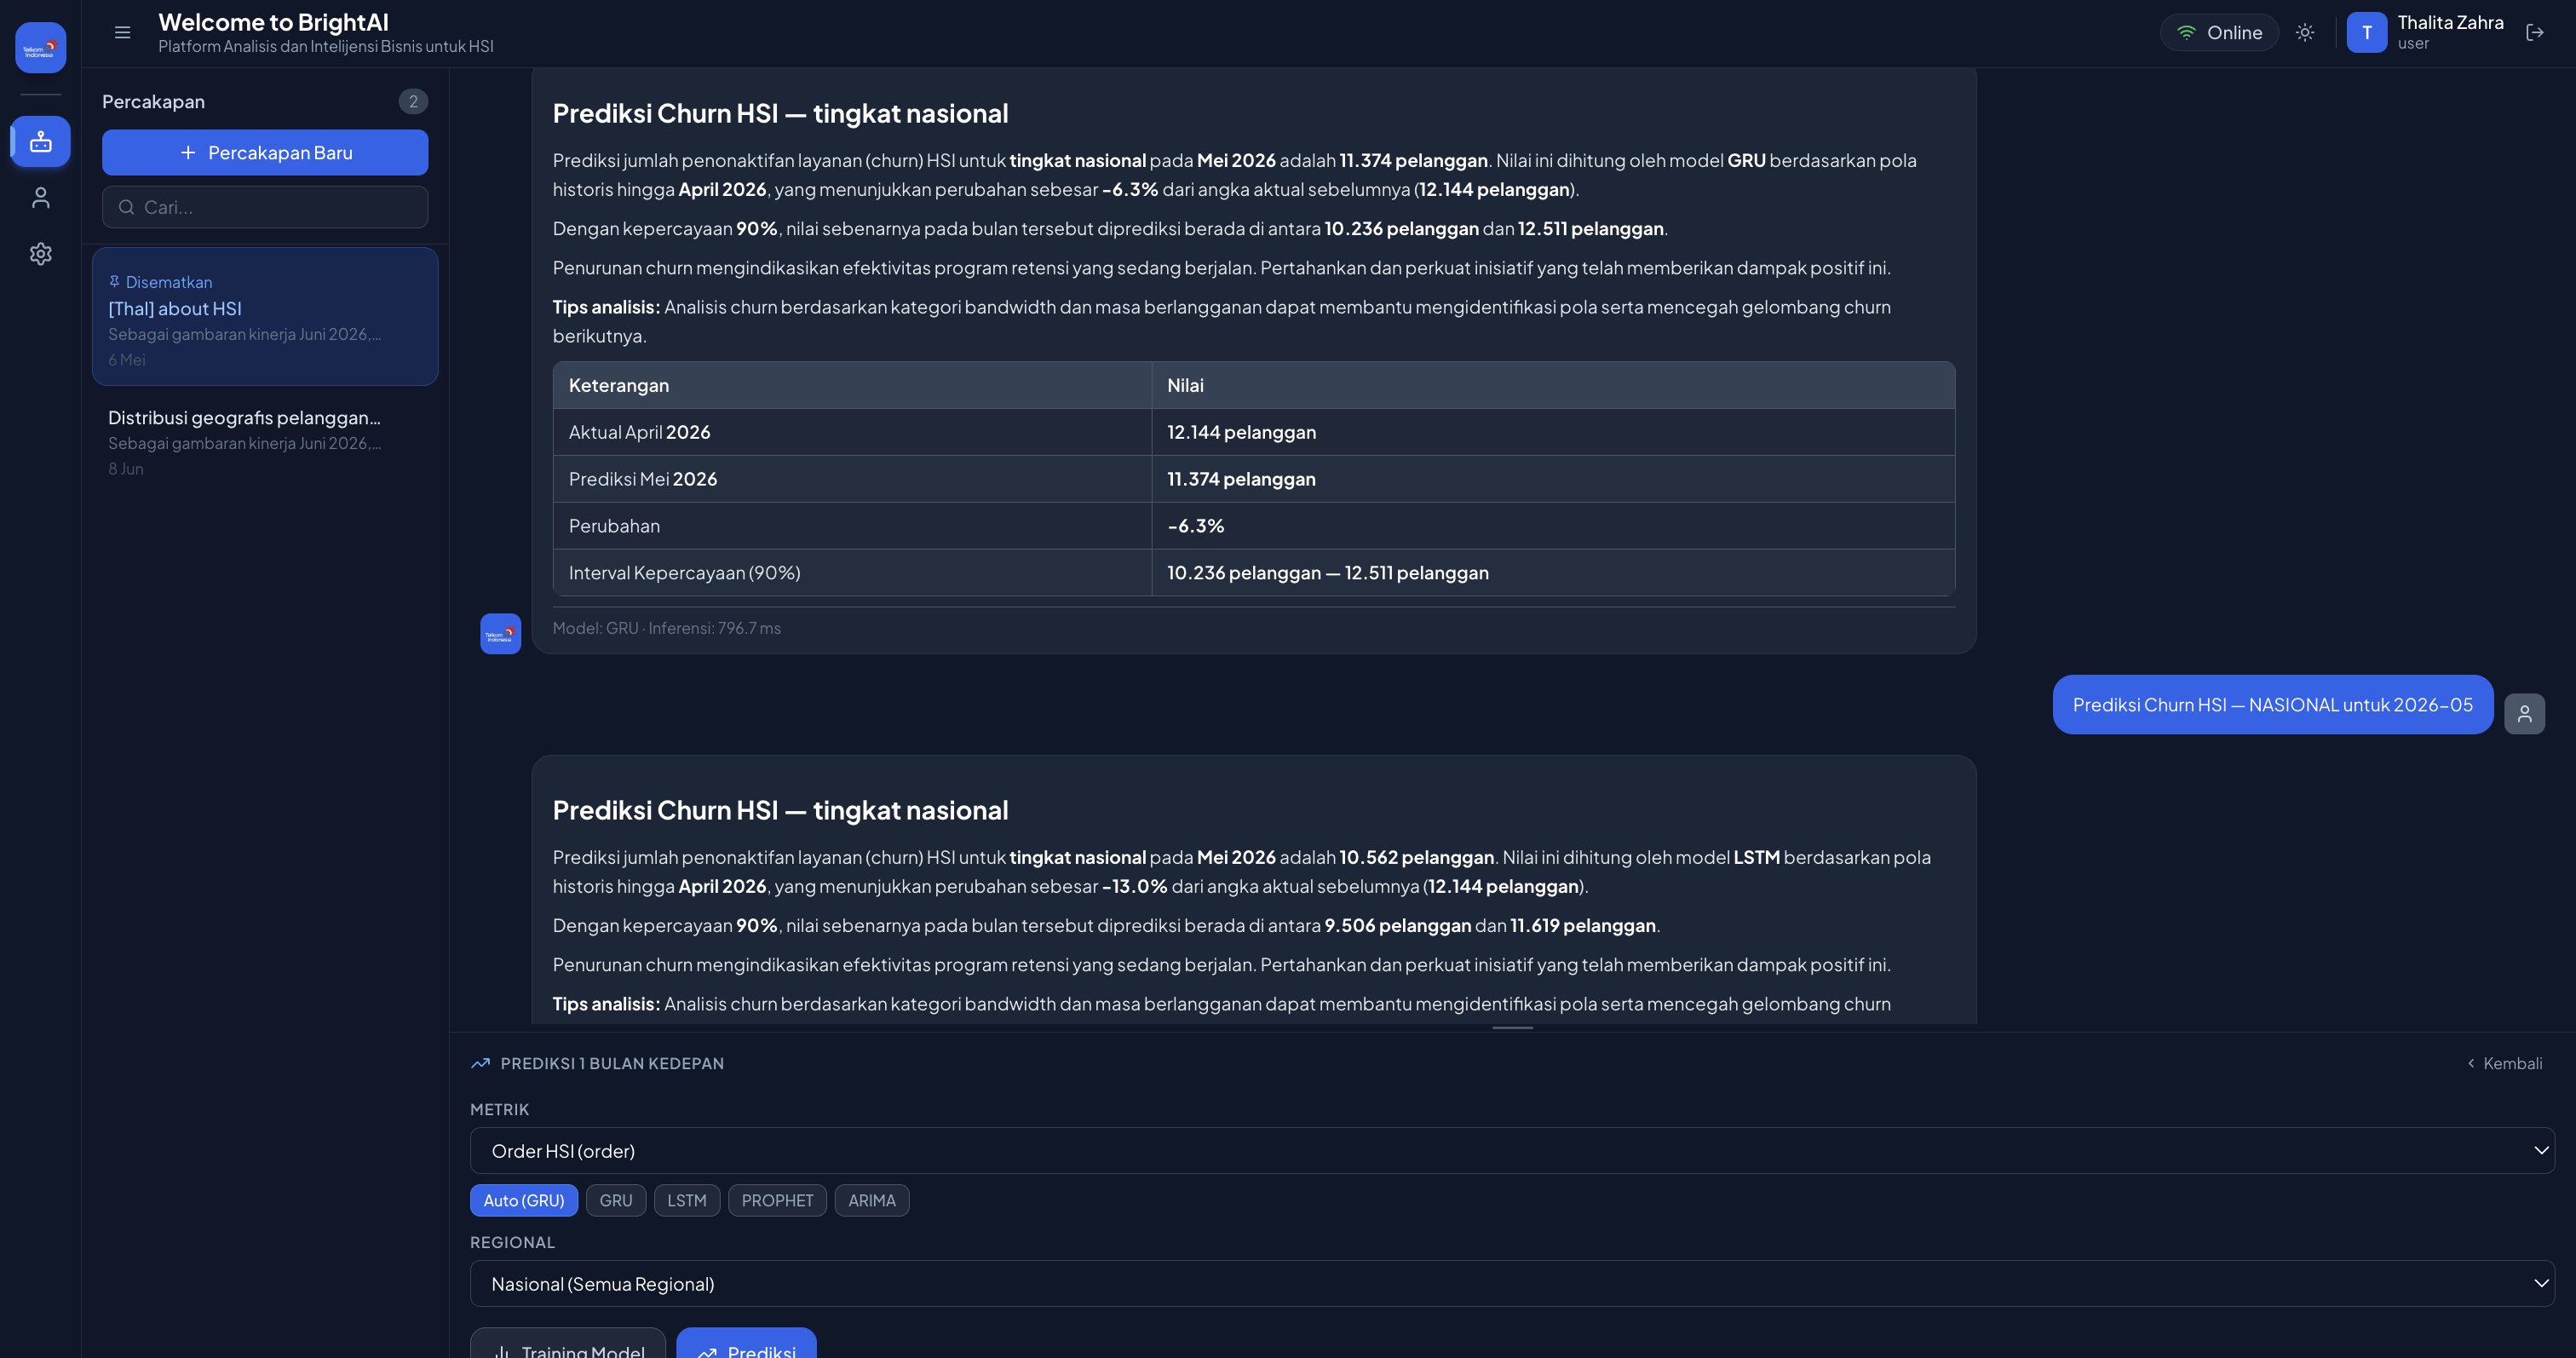
\includegraphics[width=0.85\textwidth]{images/imagemockup8}
\caption{Contoh Hasil Peramalan Deret Waktu melalui Panel \textit{Forecast}}
\label{fig:ui-forecast}
\end{figure}

Sistem terhubung ke Oracle Database melalui dua skema: \texttt{DWH\_MOIS} untuk data analitik dan \texttt{USR\_RPT} untuk data operasional. Sistem menggunakan mekanisme \textit{caching} memori untuk mengoptimalkan waktu respons. Injeksi filter geografis secara dinamis memungkinkan sistem menyajikan analisis pada tingkat nasional, regional, maupun \textit{witel} tanpa duplikasi definisi aturan.

\subsection{Selisih antara Rancangan dan Implementasi}
\label{subsec:selisih-rancangan-implementasi}

Demi transparansi, bagian ini menyatakan secara eksplisit selisih antara komponen yang dirancang pada Bab~\ref{chap:perancangan} dan komponen yang berhasil diimplementasikan. Tabel~\ref{tab:selisih-impl} merangkum selisih tersebut.

\begin{table}[h]
\centering
\caption{Selisih antara Rancangan dan Implementasi}
\label{tab:selisih-impl}
\begin{tabular}{|p{3.5cm}|p{3cm}|p{6cm}|}
\hline
\textbf{Komponen} & \textbf{Status} & \textbf{Keterangan} \\
\hline
\textit{Temporal Fusion Transformer} (TFT) & Tidak diimplementasikan & Dikaji dalam studi literatur (Subbab~\ref{subsec:tft-literatur}) sebagai arsitektur lanjutan, namun tidak termasuk dalam lingkup implementasi penelitian ini karena keterbatasan volume data dan biaya komputasi. TFT tetap menjadi kandidat pengembangan di masa depan. \\
\hline
Model \textit{ensemble} (gabungan keluaran beberapa model) & Tidak diimplementasikan & Dibahas secara teoretis pada kajian literatur, namun implementasi saat ini menjalankan setiap model secara independen tanpa mekanisme penggabungan prediksi. \\
\hline
Komponen hari libur pada \textit{Prophet} & Diimplementasikan sebagian & Daftar hari libur Indonesia telah didefinisikan dalam kode, namun dampaknya terbatas karena data bersifat bulanan sehingga efek hari libur tidak dominan. \\
\hline
\end{tabular}
\end{table}

Selain ketiga komponen di atas, seluruh rancangan yang ditetapkan pada Bab~\ref{chap:perancangan} telah berhasil diwujudkan dalam implementasi, meliputi mesin aturan (38 aturan, 5 domain), klasifikasi maksud (7 kategori \textit{intent} dan 1 \textit{fallback}), pembangkitan bahasa alami berbasis templat, model peramalan GRU dan LSTM beserta \textit{baseline} ARIMA dan \textit{Prophet}, autentikasi berbasis JWT, serta antarmuka percakapan interaktif.
